\documentclass{article}

\usepackage{noweb}
\noweboptions{smallcode,longchunks}

\usepackage[a4paper,margin=1in]{geometry}

\usepackage{adjustbox}
\usepackage{amsmath}
\usepackage{amssymb}
\usepackage{amsthm}
\usepackage{colortbl}
\usepackage{enumitem}
\usepackage[colorlinks=true]{hyperref}
\usepackage{multicol}
\usepackage{multirow}
\usepackage{tikz}

% Define a handy paragraph opener
\newcommand{\hi}[1]{\noindent {\bf #1}}

% Remove noweb page break penalty
\def\nwendcode{\endtrivlist \endgroup}
\let\nwdocspar=\par

% Define an "example" environment
\theoremstyle{definition}
\newtheorem{example}{Example}

% Define colors for tables
\definecolor{TableTitle}{rgb}{0.900, 0.900, 0.900}
\definecolor{TableHeader}{rgb}{0.900, 0.900, 0.900}

\title{Jargo's Storage Interface
  and Data Model\footnote{\url{https://github.com/jargors/Storage}}\\
  \vspace{.5em}
  \Large{\textbf{Correctness Test Program}}}
\author{James J. Pan\\
  \small{\href{mailto:jamesjpan@outlook.com}{jamesjpan@outlook.com}}
}

\begin{document}
\maketitle
\pagestyle{noweb}

\begin{figure}[h]
\centering
\fbox{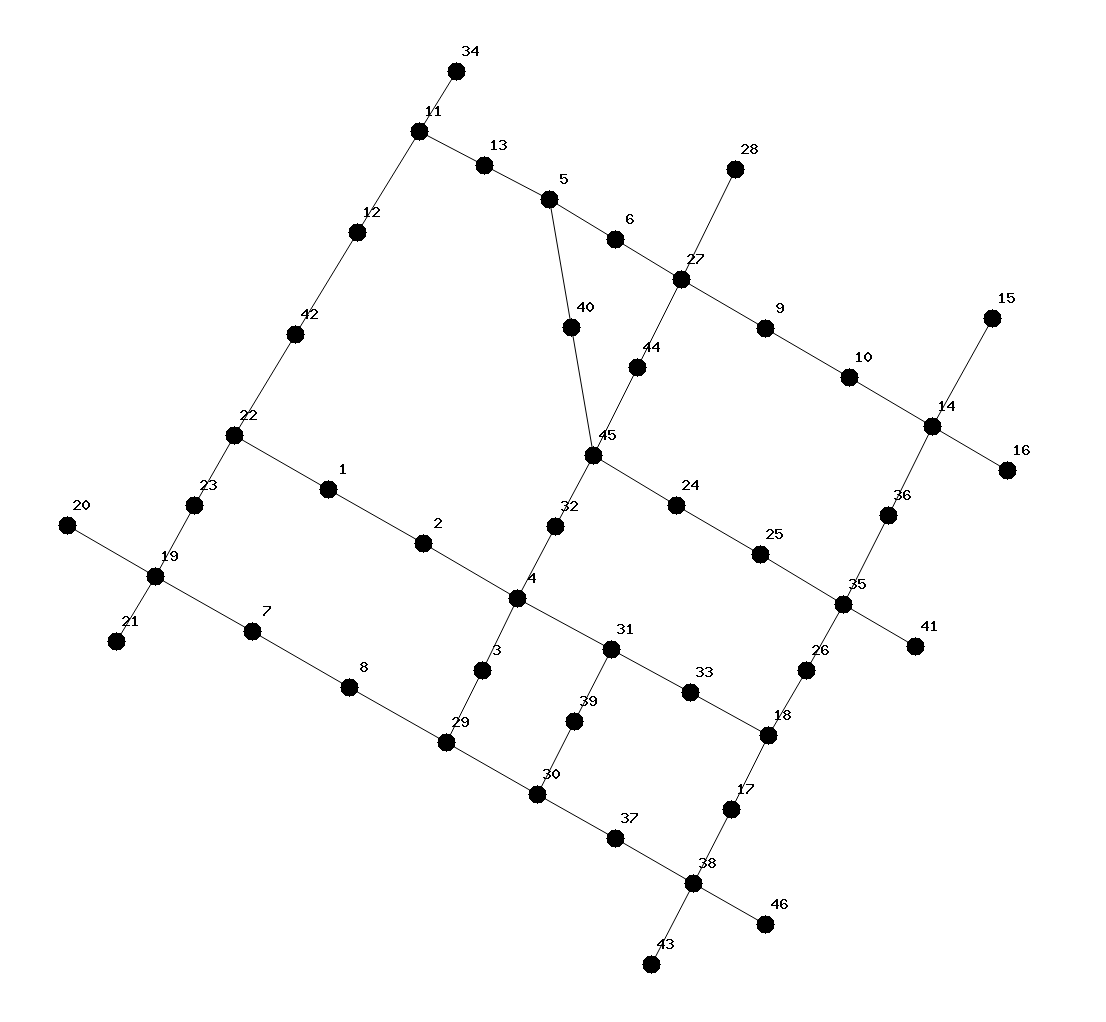
\includegraphics[width=\textwidth]{data/small-directed-dummy.png}}
\caption{Portion of a road network in Chengdu, China,
    used for tests (46 nodes, 104 directed edges).}
\label{fig:road-network}
\end{figure}
\newpage

\tableofcontents

\section{Introduction}
\label{sec:introduction}
The correctness test program for Jargo's storage interface uses a series of
positive tests to check that the storage interface is functioning correctly.
These tests pass if the output from the storage interface matches with what is
expected. A database storing a test ridesharing state is provided in
{\tt{}data/db}.  The test road network is shown in Figure~\ref{fig:road-network}.
The vertex coordinates can be found in {\tt{}data/small-directed-dummy.rnet}.
Keep in mind that the tests are not comprehensive and do not guarantee bug-free
code. Not all possible inputs to the storage interface methods are tested,
although more comprehensive testing may be added in the future.
The test program is developed using the
Noweb\footnote{\url{https://www.cs.tufts.edu/~nr/noweb/}} literate
programming\footnote{\url{http://literateprogramming.com/}} tool.  This file
({\tt{}src/storagetest.nw}) is the source for both the documentation
({\tt{}doc/storagetest.tex}) and the Java code (StorageTest.java)\footnote{See the
{\tt{}Makefile} for build details.}.
\nwfilename{src/storagetest.nw}\nwbegincode{1}\sublabel{NW2VbIVs-4CXNcc-1}\nwmargintag{{\nwtagstyle{}\subpageref{NW2VbIVs-4CXNcc-1}}}\moddef{StorageTest.java~{\nwtagstyle{}\subpageref{NW2VbIVs-4CXNcc-1}}}\endmoddef\nwnotused{StorageTest.java}
  \LA{}StorageTest.java preamble~{\nwtagstyle{}\subpageref{NW2VbIVs-2FnbX5-1}}\RA{}
  \LA{}\code{}StorageTest\edoc{} definition~{\nwtagstyle{}\subpageref{NW2VbIVs-2FrK1x-1}}\RA{}
\nwendcode{}\nwbegindocs{2}\nwdocspar

\nwenddocs{}\nwbegincode{3}\sublabel{NW2VbIVs-2FnbX5-1}\nwmargintag{{\nwtagstyle{}\subpageref{NW2VbIVs-2FnbX5-1}}}\moddef{StorageTest.java preamble~{\nwtagstyle{}\subpageref{NW2VbIVs-2FnbX5-1}}}\endmoddef\nwused{\\{NW2VbIVs-4CXNcc-1}}
import com.github.jargors.Storage;
import java.time.LocalDateTime;
\nwendcode{}\nwbegindocs{4}\nwdocspar
\nwenddocs{}\nwbegincode{5}\sublabel{NW2VbIVs-2FrK1x-1}\nwmargintag{{\nwtagstyle{}\subpageref{NW2VbIVs-2FrK1x-1}}}\moddef{\code{}StorageTest\edoc{} definition~{\nwtagstyle{}\subpageref{NW2VbIVs-2FrK1x-1}}}\endmoddef\nwused{\\{NW2VbIVs-4CXNcc-1}}
public class StorageTest \{
  \LA{}\code{}StorageTest\edoc{} member variables~{\nwtagstyle{}\subpageref{NW2VbIVs-1bhd99-1}}\RA{}
  \LA{}\code{}StorageTest\edoc{} main routine~{\nwtagstyle{}\subpageref{NW2VbIVs-2NJ9Wq-1}}\RA{}
  \LA{}\code{}StorageTest\edoc{} private methods~{\nwtagstyle{}\subpageref{NW2VbIVs-4WIMB3-1}}\RA{}
\}
\nwendcode{}\nwbegindocs{6}\nwdocspar
\nwenddocs{}\nwbegincode{7}\sublabel{NW2VbIVs-1bhd99-1}\nwmargintag{{\nwtagstyle{}\subpageref{NW2VbIVs-1bhd99-1}}}\moddef{\code{}StorageTest\edoc{} member variables~{\nwtagstyle{}\subpageref{NW2VbIVs-1bhd99-1}}}\endmoddef\nwused{\\{NW2VbIVs-2FrK1x-1}}
private static int count_passed = 0;
private static int count_failed = 0;
\nwindexdefn{count{\char95}passed}{count:unpassed}{NW2VbIVs-1bhd99-1}\nwindexdefn{count{\char95}failed}{count:unfailed}{NW2VbIVs-1bhd99-1}\eatline
\nwidentdefs{\\{{count{\char95}failed}{count:unfailed}}\\{{count{\char95}passed}{count:unpassed}}}\nwendcode{}\nwbegincode{8}\sublabel{NW2VbIVs-2NJ9Wq-1}\nwmargintag{{\nwtagstyle{}\subpageref{NW2VbIVs-2NJ9Wq-1}}}\moddef{\code{}StorageTest\edoc{} main routine~{\nwtagstyle{}\subpageref{NW2VbIVs-2NJ9Wq-1}}}\endmoddef\nwused{\\{NW2VbIVs-2FrK1x-1}}
public static void main(String[] args) \{
  Print("Starting storage interface tests");
  Storage storage = new Storage("data/small-directed-dummy.rnet");
  \LA{}..load test database~{\nwtagstyle{}\subpageref{NW2VbIVs-11CmW8-1}}\RA{}
  \LA{}..run read tests~{\nwtagstyle{}\subpageref{NW2VbIVs-2w6SyW-1}}\RA{}
  \LA{}..run write tests~{\nwtagstyle{}\subpageref{NW2VbIVs-4HcfWS-1}}\RA{}
  Print("Complete! Passed: "+count_passed+"; Failed: "+count_failed);
\}
\nwindexdefn{main}{main}{NW2VbIVs-2NJ9Wq-1}\eatline
\nwidentdefs{\\{{main}{main}}}\nwidentuses{\\{{count{\char95}failed}{count:unfailed}}\\{{count{\char95}passed}{count:unpassed}}}\nwindexuse{count{\char95}failed}{count:unfailed}{NW2VbIVs-2NJ9Wq-1}\nwindexuse{count{\char95}passed}{count:unpassed}{NW2VbIVs-2NJ9Wq-1}\nwendcode{}\nwbegindocs{9}We load a manually prepared test database.
\nwenddocs{}\nwbegincode{10}\sublabel{NW2VbIVs-11CmW8-1}\nwmargintag{{\nwtagstyle{}\subpageref{NW2VbIVs-11CmW8-1}}}\moddef{..load test database~{\nwtagstyle{}\subpageref{NW2VbIVs-11CmW8-1}}}\endmoddef\nwused{\\{NW2VbIVs-2NJ9Wq-1}}
storage.DBLoadBackup("data/db");
\nwendcode{}\nwbegindocs{11}\nwdocspar
\nwenddocs{}\nwbegincode{12}\sublabel{NW2VbIVs-4WIMB3-1}\nwmargintag{{\nwtagstyle{}\subpageref{NW2VbIVs-4WIMB3-1}}}\moddef{\code{}StorageTest\edoc{} private methods~{\nwtagstyle{}\subpageref{NW2VbIVs-4WIMB3-1}}}\endmoddef\nwused{\\{NW2VbIVs-2FrK1x-1}}
private static void Print(String msg) \{
  System.out.println("[StorageTest]["+LocalDateTime.now()+"] "+msg);
\}
\nwendcode{}\nwbegindocs{13}\nwdocspar

\section{Tests}
\label{sec:tests}

\subsection{Read Tests}
\label{sec:read-tests}
\nwenddocs{}\nwbegincode{14}\sublabel{NW2VbIVs-2w6SyW-1}\nwmargintag{{\nwtagstyle{}\subpageref{NW2VbIVs-2w6SyW-1}}}\moddef{..run read tests~{\nwtagstyle{}\subpageref{NW2VbIVs-2w6SyW-1}}}\endmoddef\nwused{\\{NW2VbIVs-2NJ9Wq-1}}
\LA{}....test \code{}DBQuery\edoc{}(2)~{\nwtagstyle{}\subpageref{NW2VbIVs-RMkGl-1}}\RA{}
\LA{}....test \code{}DBQueryServer\edoc{}(1)~{\nwtagstyle{}\subpageref{NW2VbIVs-3O8MFc-1}}\RA{}
\LA{}....test \code{}DBQueryRequest\edoc{}(1)~{\nwtagstyle{}\subpageref{NW2VbIVs-1C0pk3-1}}\RA{}
\LA{}....test \code{}DBQueryQueuedRequests\edoc{}(1)~{\nwtagstyle{}\subpageref{NW2VbIVs-1Ao9lm-1}}\RA{}
\LA{}....test \code{}DBQueryServerLocationsAll\edoc{}(1)~{\nwtagstyle{}\subpageref{NW2VbIVs-2dAmyn-1}}\RA{}
\LA{}....test \code{}DBQueryServerLocationsActive\edoc{}(1)~{\nwtagstyle{}\subpageref{NW2VbIVs-3GrgPk-1}}\RA{}
\LA{}....test \code{}DBQueryRoute\edoc{}(1)~{\nwtagstyle{}\subpageref{NW2VbIVs-4TWZqG-1}}\RA{}
\LA{}....test \code{}DBQueryRouteRemaining\edoc{}(2)~{\nwtagstyle{}\subpageref{NW2VbIVs-1LMBE6-1}}\RA{}
\LA{}....test \code{}DBQuerySchedule\edoc{}(1)~{\nwtagstyle{}\subpageref{NW2VbIVs-3I1Rij-1}}\RA{}
\LA{}....test \code{}DBQueryScheduleRemaining\edoc{}(2)~{\nwtagstyle{}\subpageref{NW2VbIVs-3vhAZd-1}}\RA{}
\LA{}....test \code{}DBQueryCurrentLoad\edoc{}(2)~{\nwtagstyle{}\subpageref{NW2VbIVs-2jSLg0-1}}\RA{}
\LA{}....test \code{}DBQueryCountVertices\edoc{}(0)~{\nwtagstyle{}\subpageref{NW2VbIVs-2FbhMk-1}}\RA{}
\LA{}....test \code{}DBQueryCountEdges\edoc{}(0)~{\nwtagstyle{}\subpageref{NW2VbIVs-fMEma-1}}\RA{}
\LA{}....test \code{}DBQueryVertex\edoc{}(1)~{\nwtagstyle{}\subpageref{NW2VbIVs-HmHFv-1}}\RA{}
\LA{}....test \code{}DBQueryEdge\edoc{}(2)~{\nwtagstyle{}\subpageref{NW2VbIVs-4e874K-1}}\RA{}
\LA{}....test \code{}DBQueryStatisticsEdges\edoc{}(0)~{\nwtagstyle{}\subpageref{NW2VbIVs-3wfpeD-1}}\RA{}
\LA{}....test \code{}DBQueryMBR\edoc{}(0)~{\nwtagstyle{}\subpageref{NW2VbIVs-2Yf5B8-1}}\RA{}
\LA{}....test \code{}DBQueryCountServers\edoc{}(0)~{\nwtagstyle{}\subpageref{NW2VbIVs-2qdA7h-1}}\RA{}
\LA{}....test \code{}DBQueryCountRequests\edoc{}(0)~{\nwtagstyle{}\subpageref{NW2VbIVs-3azEeu-1}}\RA{}
\LA{}....test \code{}DBQueryServerPendingAssignments\edoc{}(2)~{\nwtagstyle{}\subpageref{NW2VbIVs-g6QHQ-1}}\RA{}
\LA{}....test \code{}DBQueryServerCompletedAssignments\edoc{}(2)~{\nwtagstyle{}\subpageref{NW2VbIVs-1HkuSf-1}}\RA{}
\LA{}....test \code{}DBQueryServiceRate\edoc{}(0)~{\nwtagstyle{}\subpageref{NW2VbIVs-3JCT8W-1}}\RA{}
\LA{}....test \code{}DBQueryBaseDistanceTotal\edoc{}(0)~{\nwtagstyle{}\subpageref{NW2VbIVs-3FE8t4-1}}\RA{}
\LA{}....test \code{}DBQueryServerBaseDistanceTotal\edoc{}(0)~{\nwtagstyle{}\subpageref{NW2VbIVs-1BF5dX-1}}\RA{}
\LA{}....test \code{}DBQueryRequestBaseDistanceTotal\edoc{}(0)~{\nwtagstyle{}\subpageref{NW2VbIVs-38E973-1}}\RA{}
\LA{}....test \code{}DBQueryServerTravelDistance\edoc{}(1)~{\nwtagstyle{}\subpageref{NW2VbIVs-R0me6-1}}\RA{}
\LA{}....test \code{}DBQueryServerTravelDistanceTotal\edoc{}(0)~{\nwtagstyle{}\subpageref{NW2VbIVs-2cvcHE-1}}\RA{}
\LA{}....test \code{}DBQueryServerCruisingDistance\edoc{}(1)~{\nwtagstyle{}\subpageref{NW2VbIVs-okQ1Q-1}}\RA{}
\LA{}....test \code{}DBQueryServerCruisingDistanceTotal\edoc{}(0)~{\nwtagstyle{}\subpageref{NW2VbIVs-1RB1yH-1}}\RA{}
\LA{}....test \code{}DBQueryServerServiceDistance\edoc{}(1)~{\nwtagstyle{}\subpageref{NW2VbIVs-3T7Ecl-1}}\RA{}
\LA{}....test \code{}DBQueryServerServiceDistanceTotal\edoc{}(0)~{\nwtagstyle{}\subpageref{NW2VbIVs-2c14Sj-1}}\RA{}
\LA{}....test \code{}DBQueryRequestDetourDistance\edoc{}(1)~{\nwtagstyle{}\subpageref{NW2VbIVs-sBkzR-1}}\RA{}
\LA{}....test \code{}DBQueryRequestDetourDistanceTotal\edoc{}(0)~{\nwtagstyle{}\subpageref{NW2VbIVs-1qIOK3-1}}\RA{}
\LA{}....test \code{}DBQueryRequestTransitDistance\edoc{}(1)~{\nwtagstyle{}\subpageref{NW2VbIVs-3yzPUp-1}}\RA{}
\LA{}....test \code{}DBQueryRequestTransitDistanceTotal\edoc{}(0)~{\nwtagstyle{}\subpageref{NW2VbIVs-NiwSo-1}}\RA{}
\LA{}....test \code{}DBQueryServerTravelDuration\edoc{}(1)~{\nwtagstyle{}\subpageref{NW2VbIVs-1TZ4V8-1}}\RA{}
\LA{}....test \code{}DBQueryServerTravelDurationTotal\edoc{}(0)~{\nwtagstyle{}\subpageref{NW2VbIVs-2bE0DP-1}}\RA{}
\LA{}....test \code{}DBQueryRequestPickupDuration\edoc{}(1)~{\nwtagstyle{}\subpageref{NW2VbIVs-2weSRk-1}}\RA{}
\LA{}....test \code{}DBQueryRequestPickupDurationTotal\edoc{}(0)~{\nwtagstyle{}\subpageref{NW2VbIVs-PC7q9-1}}\RA{}
\LA{}....test \code{}DBQueryRequestTransitDuration\edoc{}(1)~{\nwtagstyle{}\subpageref{NW2VbIVs-2uQ1SB-1}}\RA{}
\LA{}....test \code{}DBQueryRequestTransitDurationTotal\edoc{}(0)~{\nwtagstyle{}\subpageref{NW2VbIVs-PQhaD-1}}\RA{}
\LA{}....test \code{}DBQueryRequestTravelDuration\edoc{}(1)~{\nwtagstyle{}\subpageref{NW2VbIVs-4MzTFA-1}}\RA{}
\LA{}....test \code{}DBQueryRequestTravelDurationTotal\edoc{}(0)~{\nwtagstyle{}\subpageref{NW2VbIVs-ALSer-1}}\RA{}
\LA{}....test \code{}DBQueryRequestDepartureTime\edoc{}(1)~{\nwtagstyle{}\subpageref{NW2VbIVs-XFEEZ-1}}\RA{}
\LA{}....test \code{}DBQueryServerDepartureTime\edoc{}(1)~{\nwtagstyle{}\subpageref{NW2VbIVs-1TCj44-1}}\RA{}
\LA{}....test \code{}DBQueryRequestArrivalTime\edoc{}(1)~{\nwtagstyle{}\subpageref{NW2VbIVs-1dQ6qD-1}}\RA{}
\LA{}....test \code{}DBQueryServerArrivalTime\edoc{}(1)~{\nwtagstyle{}\subpageref{NW2VbIVs-1angPN-1}}\RA{}
\nwendcode{}\nwbegindocs{15}\nwdocspar

\subsubsection{{\tt{}DBQuery}(2)}
Test {\tt{}DBQuery}(2) with a simple select statement. The road network has
46 vertices, plus 1 dummy vertex for a total of 47 vertices.
\nwenddocs{}\nwbegincode{16}\sublabel{NW2VbIVs-RMkGl-1}\nwmargintag{{\nwtagstyle{}\subpageref{NW2VbIVs-RMkGl-1}}}\moddef{....test \code{}DBQuery\edoc{}(2)~{\nwtagstyle{}\subpageref{NW2VbIVs-RMkGl-1}}}\endmoddef\nwused{\\{NW2VbIVs-2w6SyW-1}}
\{
  int output[] = storage.DBQuery("SELECT COUNT (*) FROM V", 1);
  if (output[0] != 47) \{
    Print("[FAIL] DBQuery(2)");
    Print("\\tExpected 47; got "+output[0]);
    count_failed++;
  \} else \{
    Print("[PASS] DBQuery(2)");
    count_passed++;
  \}
\}
\nwidentuses{\\{{count{\char95}failed}{count:unfailed}}\\{{count{\char95}passed}{count:unpassed}}}\nwindexuse{count{\char95}failed}{count:unfailed}{NW2VbIVs-RMkGl-1}\nwindexuse{count{\char95}passed}{count:unpassed}{NW2VbIVs-RMkGl-1}\nwendcode{}\nwbegindocs{17}\nwdocspar

\subsubsection{{\tt{}DBQueryServer}(1)}
\nwenddocs{}\nwbegincode{18}\sublabel{NW2VbIVs-3O8MFc-1}\nwmargintag{{\nwtagstyle{}\subpageref{NW2VbIVs-3O8MFc-1}}}\moddef{....test \code{}DBQueryServer\edoc{}(1)~{\nwtagstyle{}\subpageref{NW2VbIVs-3O8MFc-1}}}\endmoddef\nwused{\\{NW2VbIVs-2w6SyW-1}}
\{
  int output[] = storage.DBQueryServer(1);
  if (!(output[0] == 1
     && output[1] == -10
     && output[2] == 1
     && output[3] == 500
     && output[4] == 22
     && output[5] == 0
     && output[6] == 0)) \{
    Print("[FAIL] DBQueryServer(1)");
    Print("\\tExpected \{uid=1, q=-10, e=1, l=500, o=22, d=0, b=0\}; got");
    storage.printUser(output);
    count_failed++;
  \} else \{
    Print("[PASS] DBQueryServer(1)");
    count_passed++;
  \}
\}
\nwidentuses{\\{{count{\char95}failed}{count:unfailed}}\\{{count{\char95}passed}{count:unpassed}}}\nwindexuse{count{\char95}failed}{count:unfailed}{NW2VbIVs-3O8MFc-1}\nwindexuse{count{\char95}passed}{count:unpassed}{NW2VbIVs-3O8MFc-1}\nwendcode{}\nwbegindocs{19}\nwdocspar
\subsubsection{{\tt{}DBQueryRequest}(1)}
\nwenddocs{}\nwbegincode{20}\sublabel{NW2VbIVs-1C0pk3-1}\nwmargintag{{\nwtagstyle{}\subpageref{NW2VbIVs-1C0pk3-1}}}\moddef{....test \code{}DBQueryRequest\edoc{}(1)~{\nwtagstyle{}\subpageref{NW2VbIVs-1C0pk3-1}}}\endmoddef\nwused{\\{NW2VbIVs-2w6SyW-1}}
\{
  int output[] = storage.DBQueryRequest(10);
  if (!(output[0] == 10
     && output[1] == 1
     && output[2] == 0
     && output[3] == 500
     && output[4] == 4
     && output[5] == 30
     && output[6] == 172)) \{
    Print("[FAIL] DBQueryRequest(1)");
    Print("\\tExpected \{uid=10, q=1, e=0, l=500, o=4, d=30, b=172\}; got");
    storage.printUser(output);
    count_failed++;
  \} else \{
    Print("[PASS] DBQueryRequest(1)");
    count_passed++;
  \}
\}
\nwidentuses{\\{{count{\char95}failed}{count:unfailed}}\\{{count{\char95}passed}{count:unpassed}}}\nwindexuse{count{\char95}failed}{count:unfailed}{NW2VbIVs-1C0pk3-1}\nwindexuse{count{\char95}passed}{count:unpassed}{NW2VbIVs-1C0pk3-1}\nwendcode{}\nwbegindocs{21}\nwdocspar
\subsubsection{{\tt{}DBQueryQueuedRequests}(1)}
In the test database, Request 11 is never assigned. It appears
at $t=5$ and times out after $t=35$.
\nwenddocs{}\nwbegincode{22}\sublabel{NW2VbIVs-1Ao9lm-1}\nwmargintag{{\nwtagstyle{}\subpageref{NW2VbIVs-1Ao9lm-1}}}\moddef{....test \code{}DBQueryQueuedRequests\edoc{}(1)~{\nwtagstyle{}\subpageref{NW2VbIVs-1Ao9lm-1}}}\endmoddef\nwused{\\{NW2VbIVs-2w6SyW-1}}
\{
  \LA{}......test \code{}DBQueryQueuedRequests\edoc{}(1) at t=0~{\nwtagstyle{}\subpageref{NW2VbIVs-2K5XSE-1}}\RA{}
  \LA{}......test \code{}DBQueryQueuedRequests\edoc{}(1) at t=5~{\nwtagstyle{}\subpageref{NW2VbIVs-3LO5Sc-1}}\RA{}
  \LA{}......test \code{}DBQueryQueuedRequests\edoc{}(1) at t=35~{\nwtagstyle{}\subpageref{NW2VbIVs-3GJyuc-1}}\RA{}
  \LA{}......test \code{}DBQueryQueuedRequests\edoc{}(1) at t=36~{\nwtagstyle{}\subpageref{NW2VbIVs-182uIY-1}}\RA{}
\}
\nwendcode{}\nwbegindocs{23}\nwdocspar
As Request 11 has not appeared yet at $t=0$, we expect
{\tt{}DBQueryQueuedRequests} to return nothing.
\nwenddocs{}\nwbegincode{24}\sublabel{NW2VbIVs-2K5XSE-1}\nwmargintag{{\nwtagstyle{}\subpageref{NW2VbIVs-2K5XSE-1}}}\moddef{......test \code{}DBQueryQueuedRequests\edoc{}(1) at t=0~{\nwtagstyle{}\subpageref{NW2VbIVs-2K5XSE-1}}}\endmoddef\nwused{\\{NW2VbIVs-1Ao9lm-1}}
\{
  int output[] = storage.DBQueryQueuedRequests(0);
  if (!(output.length/7 == 0)) \{
    Print("[FAIL] DBQueryQueuedRequests(1) (1/4)");
    Print("\\tExpected 0; got "+output.length/7);
    count_failed++;
  \} else \{
    Print("[PASS] DBQueryQueuedRequests(1) (1/4)");
    count_passed++;
  \}
\}
\nwidentuses{\\{{count{\char95}failed}{count:unfailed}}\\{{count{\char95}passed}{count:unpassed}}}\nwindexuse{count{\char95}failed}{count:unfailed}{NW2VbIVs-2K5XSE-1}\nwindexuse{count{\char95}passed}{count:unpassed}{NW2VbIVs-2K5XSE-1}\nwendcode{}\nwbegindocs{25}\nwdocspar
At $t=5$, Request 11 should have just appeared and be queued up.
\nwenddocs{}\nwbegincode{26}\sublabel{NW2VbIVs-3LO5Sc-1}\nwmargintag{{\nwtagstyle{}\subpageref{NW2VbIVs-3LO5Sc-1}}}\moddef{......test \code{}DBQueryQueuedRequests\edoc{}(1) at t=5~{\nwtagstyle{}\subpageref{NW2VbIVs-3LO5Sc-1}}}\endmoddef\nwused{\\{NW2VbIVs-1Ao9lm-1}}
\{
  int output[] = storage.DBQueryQueuedRequests(5);
  if (!(output.length/7 == 1)) \{
    Print("[FAIL] DBQueryQueuedRequests(1) (2/4)");
    Print("\\tExpected 1; got "+output.length/7);
    count_failed++;
  \} else if (!(output[0] == 11)
    && (output[1] == 1)
    && (output[2] == 5)
    && (output[3] == 500)
    && (output[4] == 1)
    && (output[5] == 32)
    && (output[6] == 194)) \{
    Print("[FAIL] DBQueryQueuedRequests(1) (2/4)");
    Print("\\tExpected \{uid=11, q=1, e=5, l=500, o=1, d=32, b=194\}; got");
    storage.printUser(output);
    count_failed++;
  \} else \{
    Print("[PASS] DBQueryQueuedRequests(1) (2/4)");
    count_passed++;
  \}
\}
\nwidentuses{\\{{count{\char95}failed}{count:unfailed}}\\{{count{\char95}passed}{count:unpassed}}}\nwindexuse{count{\char95}failed}{count:unfailed}{NW2VbIVs-3LO5Sc-1}\nwindexuse{count{\char95}passed}{count:unpassed}{NW2VbIVs-3LO5Sc-1}\nwendcode{}\nwbegindocs{27}\nwdocspar
At $t=35$, Request 11 should be just about to time out but still in the queue.
\nwenddocs{}\nwbegincode{28}\sublabel{NW2VbIVs-3GJyuc-1}\nwmargintag{{\nwtagstyle{}\subpageref{NW2VbIVs-3GJyuc-1}}}\moddef{......test \code{}DBQueryQueuedRequests\edoc{}(1) at t=35~{\nwtagstyle{}\subpageref{NW2VbIVs-3GJyuc-1}}}\endmoddef\nwused{\\{NW2VbIVs-1Ao9lm-1}}
\{
  int output[] = storage.DBQueryQueuedRequests(35);
  if (!(output.length/7 == 1)) \{
    Print("[FAIL] DBQueryQueuedRequests(1) (3/4)");
    Print("\\tExpected 1; got "+output.length/7);
    count_failed++;
  \} else if (!(output[0] == 11)
    && (output[1] == 1)
    && (output[2] == 5)
    && (output[3] == 500)
    && (output[4] == 1)
    && (output[5] == 32)
    && (output[6] == 194)) \{
    Print("[FAIL] DBQueryQueuedRequests(1) (3/4)");
    Print("\\tExpected \{uid=11, q=1, e=5, l=500, o=1, d=32, b=194\}; got");
    storage.printUser(output);
    count_failed++;
  \} else \{
    Print("[PASS] DBQueryQueuedRequests(1) (3/4)");
    count_passed++;
  \}
\}
\nwidentuses{\\{{count{\char95}failed}{count:unfailed}}\\{{count{\char95}passed}{count:unpassed}}}\nwindexuse{count{\char95}failed}{count:unfailed}{NW2VbIVs-3GJyuc-1}\nwindexuse{count{\char95}passed}{count:unpassed}{NW2VbIVs-3GJyuc-1}\nwendcode{}\nwbegindocs{29}\nwdocspar
At $t>35$, Request 11 should be timed out and there should be no queued
requests.
\nwenddocs{}\nwbegincode{30}\sublabel{NW2VbIVs-182uIY-1}\nwmargintag{{\nwtagstyle{}\subpageref{NW2VbIVs-182uIY-1}}}\moddef{......test \code{}DBQueryQueuedRequests\edoc{}(1) at t=36~{\nwtagstyle{}\subpageref{NW2VbIVs-182uIY-1}}}\endmoddef\nwused{\\{NW2VbIVs-1Ao9lm-1}}
\{
  int output[] = storage.DBQueryQueuedRequests(36);
  if (!(output.length/7 == 0)) \{
    Print("[FAIL] DBQueryQueuedRequests(1) (4/4)");
    Print("\\tExpected 0; got "+output.length/7);
    count_failed++;
  \} else \{
    Print("[PASS] DBQueryQueuedRequests(1) (4/4)");
    count_passed++;
  \}
\}
\nwidentuses{\\{{count{\char95}failed}{count:unfailed}}\\{{count{\char95}passed}{count:unpassed}}}\nwindexuse{count{\char95}failed}{count:unfailed}{NW2VbIVs-182uIY-1}\nwindexuse{count{\char95}passed}{count:unpassed}{NW2VbIVs-182uIY-1}\nwendcode{}\nwbegindocs{31}\nwdocspar
\subsubsection{{\tt{}DBQueryServerLocationsAll}(1)}
We focus on four cases. When $t=0$, neither service has begun service yet,
and we expect no locations to be returned. When $t=44$, Server 2 is out of
server, and Server 1 has just arrived at vertex 30. When $t=45$, Server 1
has just ended service. When $t=46$, both Server 1 and Server 2 are out of
service.
\nwenddocs{}\nwbegincode{32}\sublabel{NW2VbIVs-2dAmyn-1}\nwmargintag{{\nwtagstyle{}\subpageref{NW2VbIVs-2dAmyn-1}}}\moddef{....test \code{}DBQueryServerLocationsAll\edoc{}(1)~{\nwtagstyle{}\subpageref{NW2VbIVs-2dAmyn-1}}}\endmoddef\nwused{\\{NW2VbIVs-2w6SyW-1}}
\{
  \LA{}......test \code{}DBQueryServerLocationsAll\edoc{}(1) when $t=0$~{\nwtagstyle{}\subpageref{NW2VbIVs-2sf19g-1}}\RA{}
  \LA{}......test \code{}DBQueryServerLocationsAll\edoc{}(1) when $t=44$~{\nwtagstyle{}\subpageref{NW2VbIVs-HtL0w-1}}\RA{}
  \LA{}......test \code{}DBQueryServerLocationsAll\edoc{}(1) when $t=45$~{\nwtagstyle{}\subpageref{NW2VbIVs-HH7DS-1}}\RA{}
  \LA{}......test \code{}DBQueryServerLocationsAll\edoc{}(1) when $t=46$~{\nwtagstyle{}\subpageref{NW2VbIVs-Hqj38-1}}\RA{}
\}
\nwendcode{}\nwbegindocs{33}\nwdocspar
\nwenddocs{}\nwbegincode{34}\sublabel{NW2VbIVs-2sf19g-1}\nwmargintag{{\nwtagstyle{}\subpageref{NW2VbIVs-2sf19g-1}}}\moddef{......test \code{}DBQueryServerLocationsAll\edoc{}(1) when $t=0$~{\nwtagstyle{}\subpageref{NW2VbIVs-2sf19g-1}}}\endmoddef\nwused{\\{NW2VbIVs-2dAmyn-1}}
\{
  int output[] = storage.DBQueryServerLocationsAll(0);
  if (!(output.length/3 == 0)) \{
    Print("[FAIL] DBQueryServerLocationsAll(1) (1/4)");
    Print("\\tExpected 0; got "+output.length/3);
    count_failed++;
  \} else \{
    Print("[PASS] DBQueryServerLocationsAll(1) (1/4)");
    count_passed++;
  \}
\}
\nwidentuses{\\{{count{\char95}failed}{count:unfailed}}\\{{count{\char95}passed}{count:unpassed}}}\nwindexuse{count{\char95}failed}{count:unfailed}{NW2VbIVs-2sf19g-1}\nwindexuse{count{\char95}passed}{count:unpassed}{NW2VbIVs-2sf19g-1}\nwendcode{}\nwbegindocs{35}\nwdocspar
Keep an out of for false fail due to wrong ordering that we assume out
the {\tt{}output} array.
\nwenddocs{}\nwbegincode{36}\sublabel{NW2VbIVs-HtL0w-1}\nwmargintag{{\nwtagstyle{}\subpageref{NW2VbIVs-HtL0w-1}}}\moddef{......test \code{}DBQueryServerLocationsAll\edoc{}(1) when $t=44$~{\nwtagstyle{}\subpageref{NW2VbIVs-HtL0w-1}}}\endmoddef\nwused{\\{NW2VbIVs-2dAmyn-1}}
\{
  int output[] = storage.DBQueryServerLocationsAll(44);
  if (!(output.length/3 == 2)) \{
    Print("[FAIL] DBQueryServerLocationsAll(1) (2/4)");
    Print("\\tExpected 2; got "+output.length/3);
    count_failed++;
  \} else if (!(output[0] == 1
    && output[1] == 44
    && output[2] == 30
    && output[3] == 2
    && output[4] == 28
    && output[5] == 5)) \{
    Print("[FAIL] DBQueryServerLocationsAll(1) (2/4)");
    Print("Expected (sid=1, t=44, v=30) (sid=2, t=28, v=5); got "
      + "(sid="+output[0]+", t="+output[1]+", v="+output[2]+") "
      + "(sid="+output[3]+", t="+output[4]+", v="+output[5]+")");
    count_failed++;
  \} else \{
    Print("[PASS] DBQueryServerLocationsAll(1) (2/4)");
    count_passed++;
  \}
\}
\nwidentuses{\\{{count{\char95}failed}{count:unfailed}}\\{{count{\char95}passed}{count:unpassed}}}\nwindexuse{count{\char95}failed}{count:unfailed}{NW2VbIVs-HtL0w-1}\nwindexuse{count{\char95}passed}{count:unpassed}{NW2VbIVs-HtL0w-1}\nwendcode{}\nwbegindocs{37}\nwdocspar
At $t=45$, Server 1 has just ended service and is now at the dummy vertex.
Its last known location was at vertex 30 at $t=44$. We expect to see vertex
30 returned here.
Again keep an eye out for false fail due to ordering.
\nwenddocs{}\nwbegincode{38}\sublabel{NW2VbIVs-HH7DS-1}\nwmargintag{{\nwtagstyle{}\subpageref{NW2VbIVs-HH7DS-1}}}\moddef{......test \code{}DBQueryServerLocationsAll\edoc{}(1) when $t=45$~{\nwtagstyle{}\subpageref{NW2VbIVs-HH7DS-1}}}\endmoddef\nwused{\\{NW2VbIVs-2dAmyn-1}}
\{
  int output[] = storage.DBQueryServerLocationsAll(45);
  if (!(output.length/3 == 2)) \{
    Print("[FAIL] DBQueryServerLocationsAll(1) (3/4)");
    Print("\\tExpected 2; got "+output.length/3);
    count_failed++;
  \} else if (!(output[0] == 1
    && output[1] == 44
    && output[2] == 30
    && output[3] == 2
    && output[4] == 28
    && output[5] == 5)) \{
    Print("[FAIL] DBQueryServerLocationsAll(1) (3/4)");
    Print("Expected (sid=1, t=44, v=30) (sid=2, t=28, v=5); got "
      + "(sid="+output[0]+", t="+output[1]+", v="+output[2]+") "
      + "(sid="+output[3]+", t="+output[4]+", v="+output[5]+")");
    count_failed++;
  \} else \{
    Print("[PASS] DBQueryServerLocationsAll(1) (3/4)");
    count_passed++;
  \}
\}
\nwidentuses{\\{{count{\char95}failed}{count:unfailed}}\\{{count{\char95}passed}{count:unpassed}}}\nwindexuse{count{\char95}failed}{count:unfailed}{NW2VbIVs-HH7DS-1}\nwindexuse{count{\char95}passed}{count:unpassed}{NW2VbIVs-HH7DS-1}\nwendcode{}\nwbegindocs{39}\nwdocspar
We should get the same output at $t=45$ and at $t=46$.
\nwenddocs{}\nwbegincode{40}\sublabel{NW2VbIVs-Hqj38-1}\nwmargintag{{\nwtagstyle{}\subpageref{NW2VbIVs-Hqj38-1}}}\moddef{......test \code{}DBQueryServerLocationsAll\edoc{}(1) when $t=46$~{\nwtagstyle{}\subpageref{NW2VbIVs-Hqj38-1}}}\endmoddef\nwused{\\{NW2VbIVs-2dAmyn-1}}
\{
  int output[] = storage.DBQueryServerLocationsAll(45);
  if (!(output.length/3 == 2)) \{
    Print("[FAIL] DBQueryServerLocationsAll(1) (4/4)");
    Print("\\tExpected 2; got "+output.length/3);
    count_failed++;
  \} else if (!(output[0] == 1
    && output[1] == 44
    && output[2] == 30
    && output[3] == 2
    && output[4] == 28
    && output[5] == 5)) \{
    Print("[FAIL] DBQueryServerLocationsAll(1) (4/4)");
    Print("Expected (sid=1, t=44, v=30) (sid=2, t=28, v=5); got "
      + "(sid="+output[0]+", t="+output[1]+", v="+output[2]+") "
      + "(sid="+output[3]+", t="+output[4]+", v="+output[5]+")");
    count_failed++;
  \} else \{
    Print("[PASS] DBQueryServerLocationsAll(1) (4/4)");
    count_passed++;
  \}
\}
\nwidentuses{\\{{count{\char95}failed}{count:unfailed}}\\{{count{\char95}passed}{count:unpassed}}}\nwindexuse{count{\char95}failed}{count:unfailed}{NW2VbIVs-Hqj38-1}\nwindexuse{count{\char95}passed}{count:unpassed}{NW2VbIVs-Hqj38-1}\nwendcode{}\nwbegindocs{41}\nwdocspar
\subsubsection{{\tt{}DBQueryServerLocationsActive}(1)}
\nwenddocs{}\nwbegincode{42}\sublabel{NW2VbIVs-3GrgPk-1}\nwmargintag{{\nwtagstyle{}\subpageref{NW2VbIVs-3GrgPk-1}}}\moddef{....test \code{}DBQueryServerLocationsActive\edoc{}(1)~{\nwtagstyle{}\subpageref{NW2VbIVs-3GrgPk-1}}}\endmoddef\nwused{\\{NW2VbIVs-2w6SyW-1}}
\{
  \LA{}......test \code{}DBQueryServerLocationsActive\edoc{}(1) when $t=0$~{\nwtagstyle{}\subpageref{NW2VbIVs-1JQJiP-1}}\RA{}
  \LA{}......test \code{}DBQueryServerLocationsActive\edoc{}(1) when $t=44$~{\nwtagstyle{}\subpageref{NW2VbIVs-4O1SEc-1}}\RA{}
  \LA{}......test \code{}DBQueryServerLocationsActive\edoc{}(1) when $t=45$~{\nwtagstyle{}\subpageref{NW2VbIVs-4NnQjy-1}}\RA{}
  \LA{}......test \code{}DBQueryServerLocationsActive\edoc{}(1) when $t=46$~{\nwtagstyle{}\subpageref{NW2VbIVs-4OQ470-1}}\RA{}
\}
\nwendcode{}\nwbegindocs{43}\nwdocspar
\nwenddocs{}\nwbegincode{44}\sublabel{NW2VbIVs-1JQJiP-1}\nwmargintag{{\nwtagstyle{}\subpageref{NW2VbIVs-1JQJiP-1}}}\moddef{......test \code{}DBQueryServerLocationsActive\edoc{}(1) when $t=0$~{\nwtagstyle{}\subpageref{NW2VbIVs-1JQJiP-1}}}\endmoddef\nwused{\\{NW2VbIVs-3GrgPk-1}}
\{
  int output[] = storage.DBQueryServerLocationsActive(0);
  if (!(output.length/3 == 0)) \{
    Print("[FAIL] DBQueryServerLocationsActive(1) (1/4)");
    Print("\\tExpected 0; got "+output.length/3);
    count_failed++;
  \} else \{
    Print("[PASS] DBQueryServerLocationsActive(1) (1/4)");
    count_passed++;
  \}
\}
\nwidentuses{\\{{count{\char95}failed}{count:unfailed}}\\{{count{\char95}passed}{count:unpassed}}}\nwindexuse{count{\char95}failed}{count:unfailed}{NW2VbIVs-1JQJiP-1}\nwindexuse{count{\char95}passed}{count:unpassed}{NW2VbIVs-1JQJiP-1}\nwendcode{}\nwbegindocs{45}\nwdocspar
\nwenddocs{}\nwbegincode{46}\sublabel{NW2VbIVs-4O1SEc-1}\nwmargintag{{\nwtagstyle{}\subpageref{NW2VbIVs-4O1SEc-1}}}\moddef{......test \code{}DBQueryServerLocationsActive\edoc{}(1) when $t=44$~{\nwtagstyle{}\subpageref{NW2VbIVs-4O1SEc-1}}}\endmoddef\nwused{\\{NW2VbIVs-3GrgPk-1}}
\{
  int output[] = storage.DBQueryServerLocationsActive(44);
  if (!(output.length/3 == 1)) \{
    Print("[FAIL] DBQueryServerLocationsActive(1) (2/4)");
    Print("\\tExpected 1; got "+output.length/3);
    count_failed++;
  \} else if (!(output[0] == 1
    && output[1] == 44
    && output[2] == 30)) \{
    Print("[FAIL] DBQueryServerLocationsActive(1) (2/4)");
    Print("Expected (sid=1, t=44, v=30); got "
      + "(sid="+output[0]+", t="+output[1]+", v="+output[2]+")");
    count_failed++;
  \} else \{
    Print("[PASS] DBQueryServerLocationsActive(1) (2/4)");
    count_passed++;
  \}
\}
\nwidentuses{\\{{count{\char95}failed}{count:unfailed}}\\{{count{\char95}passed}{count:unpassed}}}\nwindexuse{count{\char95}failed}{count:unfailed}{NW2VbIVs-4O1SEc-1}\nwindexuse{count{\char95}passed}{count:unpassed}{NW2VbIVs-4O1SEc-1}\nwendcode{}\nwbegindocs{47}\nwdocspar
Server 1 just ends service at $t=45$. We expect it to not appear for this
query because it is no longer active.
\nwenddocs{}\nwbegincode{48}\sublabel{NW2VbIVs-4NnQjy-1}\nwmargintag{{\nwtagstyle{}\subpageref{NW2VbIVs-4NnQjy-1}}}\moddef{......test \code{}DBQueryServerLocationsActive\edoc{}(1) when $t=45$~{\nwtagstyle{}\subpageref{NW2VbIVs-4NnQjy-1}}}\endmoddef\nwused{\\{NW2VbIVs-3GrgPk-1}}
\{
  int output[] = storage.DBQueryServerLocationsActive(45);
  if (!(output.length/3 == 0)) \{
    Print("[FAIL] DBQueryServerLocationsActive(1) (3/4)");
    Print("\\tExpected 0; got "+output.length/3);
    count_failed++;
  \} else \{
    Print("[PASS] DBQueryServerLocationsActive(1) (3/4)");
    count_passed++;
  \}
\}
\nwidentuses{\\{{count{\char95}failed}{count:unfailed}}\\{{count{\char95}passed}{count:unpassed}}}\nwindexuse{count{\char95}failed}{count:unfailed}{NW2VbIVs-4NnQjy-1}\nwindexuse{count{\char95}passed}{count:unpassed}{NW2VbIVs-4NnQjy-1}\nwendcode{}\nwbegindocs{49}\nwdocspar
\nwenddocs{}\nwbegincode{50}\sublabel{NW2VbIVs-4OQ470-1}\nwmargintag{{\nwtagstyle{}\subpageref{NW2VbIVs-4OQ470-1}}}\moddef{......test \code{}DBQueryServerLocationsActive\edoc{}(1) when $t=46$~{\nwtagstyle{}\subpageref{NW2VbIVs-4OQ470-1}}}\endmoddef\nwused{\\{NW2VbIVs-3GrgPk-1}}
\{
  int output[] = storage.DBQueryServerLocationsActive(46);
  if (!(output.length/3 == 0)) \{
    Print("[FAIL] DBQueryServerLocationsActive(1) (4/4)");
    Print("\\tExpected 0; got "+output.length/3);
    count_failed++;
  \} else \{
    Print("[PASS] DBQueryServerLocationsActive(1) (4/4)");
    count_passed++;
  \}
\}
\nwidentuses{\\{{count{\char95}failed}{count:unfailed}}\\{{count{\char95}passed}{count:unpassed}}}\nwindexuse{count{\char95}failed}{count:unfailed}{NW2VbIVs-4OQ470-1}\nwindexuse{count{\char95}passed}{count:unpassed}{NW2VbIVs-4OQ470-1}\nwendcode{}\nwbegindocs{51}\nwdocspar
\subsubsection{{\tt{}DBQueryRoute}(1)}
\nwenddocs{}\nwbegincode{52}\sublabel{NW2VbIVs-4TWZqG-1}\nwmargintag{{\nwtagstyle{}\subpageref{NW2VbIVs-4TWZqG-1}}}\moddef{....test \code{}DBQueryRoute\edoc{}(1)~{\nwtagstyle{}\subpageref{NW2VbIVs-4TWZqG-1}}}\endmoddef\nwused{\\{NW2VbIVs-2w6SyW-1}}
\{
  int output[] = storage.DBQueryRoute(2);
  if (!(output.length == 6)) \{
    Print("[FAIL] DBQueryRoute(1)");
    Print("\\tExpected 6; got "+output.length);
    count_failed++;
  \} else if (!(output[0] == 10)
    && (output[1] == 45)
    && (output[2] == 19)
    && (output[3] == 40)
    && (output[4] == 28)
    && (output[5] == 5)) \{
    Print("[FAIL] DBQueryRoute(1)");
    Print("\\tExpected (10, 45) (19, 40) (28, 5); got ");
    storage.printRoute(output);
    count_failed++;
  \} else \{
    Print("[PASS] DBQueryRoute(1)");
    count_passed++;
  \}
\}
\nwidentuses{\\{{count{\char95}failed}{count:unfailed}}\\{{count{\char95}passed}{count:unpassed}}}\nwindexuse{count{\char95}failed}{count:unfailed}{NW2VbIVs-4TWZqG-1}\nwindexuse{count{\char95}passed}{count:unpassed}{NW2VbIVs-4TWZqG-1}\nwendcode{}\nwbegindocs{53}\nwdocspar
\subsubsection{{\tt{}DBQueryRouteRemaining}(2)}
We use Server 2 to test {\tt{}DBQueryRouteRemaining}. Server 2 appears at $t=10$.
We expect the remaining route to not include its origin when $t>=10$, but
include the origin when $t<10$. Even though Server 2 is not in service when
$t<10$, we can still query its remaining route in case the simulation engine
wants to make adjustments to the route.
\nwenddocs{}\nwbegincode{54}\sublabel{NW2VbIVs-1LMBE6-1}\nwmargintag{{\nwtagstyle{}\subpageref{NW2VbIVs-1LMBE6-1}}}\moddef{....test \code{}DBQueryRouteRemaining\edoc{}(2)~{\nwtagstyle{}\subpageref{NW2VbIVs-1LMBE6-1}}}\endmoddef\nwused{\\{NW2VbIVs-2w6SyW-1}}
  \LA{}......test \code{}DBQueryRouteRemaining\edoc{}(2) at $t=9$~{\nwtagstyle{}\subpageref{NW2VbIVs-3Kf6AF-1}}\RA{}
  \LA{}......test \code{}DBQueryRouteRemaining\edoc{}(2) at $t=10$~{\nwtagstyle{}\subpageref{NW2VbIVs-3AIjLv-1}}\RA{}
  \LA{}......test \code{}DBQueryRouteRemaining\edoc{}(2) at $t=11$~{\nwtagstyle{}\subpageref{NW2VbIVs-39Mi27-1}}\RA{}
\nwendcode{}\nwbegindocs{55}\nwdocspar
\nwenddocs{}\nwbegincode{56}\sublabel{NW2VbIVs-3Kf6AF-1}\nwmargintag{{\nwtagstyle{}\subpageref{NW2VbIVs-3Kf6AF-1}}}\moddef{......test \code{}DBQueryRouteRemaining\edoc{}(2) at $t=9$~{\nwtagstyle{}\subpageref{NW2VbIVs-3Kf6AF-1}}}\endmoddef\nwused{\\{NW2VbIVs-1LMBE6-1}}
\{
  int output[] = storage.DBQueryRouteRemaining(2, 9);
  if (!(output.length == 6)) \{
    Print("[FAIL] DBQueryRouteRemaining(2) (1/3)");
    Print("\\tExpected 6; got "+output.length);
    count_failed++;
  \} else if (!(output[0] == 10
    && output[1] == 45
    && output[2] == 19
    && output[3] == 40
    && output[4] == 28
    && output[5] == 5)) \{
    Print("[FAIL] DBQueryRouteRemaining(2) (1/3)");
    Print("\\tExpected (10, 45) (19, 40) (28 5); got ");
    storage.printRoute(output);
    count_failed++;
  \} else \{
    Print("[PASS] DBQueryRouteRemaining(2) (1/3)");
    count_passed++;
  \}
\}
\nwidentuses{\\{{count{\char95}failed}{count:unfailed}}\\{{count{\char95}passed}{count:unpassed}}}\nwindexuse{count{\char95}failed}{count:unfailed}{NW2VbIVs-3Kf6AF-1}\nwindexuse{count{\char95}passed}{count:unpassed}{NW2VbIVs-3Kf6AF-1}\nwendcode{}\nwbegindocs{57}\nwdocspar
\nwenddocs{}\nwbegincode{58}\sublabel{NW2VbIVs-3AIjLv-1}\nwmargintag{{\nwtagstyle{}\subpageref{NW2VbIVs-3AIjLv-1}}}\moddef{......test \code{}DBQueryRouteRemaining\edoc{}(2) at $t=10$~{\nwtagstyle{}\subpageref{NW2VbIVs-3AIjLv-1}}}\endmoddef\nwused{\\{NW2VbIVs-1LMBE6-1}}
\{
  int output[] = storage.DBQueryRouteRemaining(2, 10);
  if (!(output.length == 4)) \{
    Print("[FAIL] DBQueryRouteRemaining(2) (2/3)");
    Print("\\tExpected 4; got "+output.length);
    count_failed++;
  \} else if (!(output[0] == 19
    && output[1] == 40
    && output[2] == 28
    && output[3] == 5)) \{
    Print("[FAIL] DBQueryRouteRemaining(2) (2/3)");
    Print("\\tExpected (19, 40) (28 5); got ");
    storage.printRoute(output);
    count_failed++;
  \} else \{
    Print("[PASS] DBQueryRouteRemaining(2) (2/3)");
    count_passed++;
  \}
\}
\nwidentuses{\\{{count{\char95}failed}{count:unfailed}}\\{{count{\char95}passed}{count:unpassed}}}\nwindexuse{count{\char95}failed}{count:unfailed}{NW2VbIVs-3AIjLv-1}\nwindexuse{count{\char95}passed}{count:unpassed}{NW2VbIVs-3AIjLv-1}\nwendcode{}\nwbegindocs{59}\nwdocspar
\nwenddocs{}\nwbegincode{60}\sublabel{NW2VbIVs-39Mi27-1}\nwmargintag{{\nwtagstyle{}\subpageref{NW2VbIVs-39Mi27-1}}}\moddef{......test \code{}DBQueryRouteRemaining\edoc{}(2) at $t=11$~{\nwtagstyle{}\subpageref{NW2VbIVs-39Mi27-1}}}\endmoddef\nwused{\\{NW2VbIVs-1LMBE6-1}}
\{
  int output[] = storage.DBQueryRouteRemaining(2, 11);
  if (!(output.length == 4)) \{
    Print("[FAIL] DBQueryRouteRemaining(2) (3/3)");
    Print("\\tExpected 4; got "+output.length);
    count_failed++;
  \} else if (!(output[0] == 19
    && output[1] == 40
    && output[2] == 28
    && output[3] == 5)) \{
    Print("[FAIL] DBQueryRouteRemaining(2) (3/3)");
    Print("\\tExpected (19, 40) (28 5); got ");
    storage.printRoute(output);
    count_failed++;
  \} else \{
    Print("[PASS] DBQueryRouteRemaining(2) (3/3)");
    count_passed++;
  \}
\}
\nwidentuses{\\{{count{\char95}failed}{count:unfailed}}\\{{count{\char95}passed}{count:unpassed}}}\nwindexuse{count{\char95}failed}{count:unfailed}{NW2VbIVs-39Mi27-1}\nwindexuse{count{\char95}passed}{count:unpassed}{NW2VbIVs-39Mi27-1}\nwendcode{}\nwbegindocs{61}\nwdocspar
\subsubsection{{\tt{}DBQuerySchedule}(1)}
\nwenddocs{}\nwbegincode{62}\sublabel{NW2VbIVs-3I1Rij-1}\nwmargintag{{\nwtagstyle{}\subpageref{NW2VbIVs-3I1Rij-1}}}\moddef{....test \code{}DBQuerySchedule\edoc{}(1)~{\nwtagstyle{}\subpageref{NW2VbIVs-3I1Rij-1}}}\endmoddef\nwused{\\{NW2VbIVs-2w6SyW-1}}
\{
  int output[] = storage.DBQuerySchedule(1);
  if (!(output.length == 16)) \{
    Print("[FAIL] DBQuerySchedule(1)");
    Print("\\tExpected 16; got "+output.length);
    count_failed++;
  \} else if (!(output[0] == 1
    && output[1] == 22
    && output[2] == 1
    && output[3] == 0
    && output[4] == 25
    && output[5] == 4
    && output[6] == 0
    && output[7] == 10
    && output[8] == 44
    && output[9] == 30
    && output[10] == 0
    && output[11] == 10
    && output[12] == 45
    && output[13] == 0
    && output[14] == 1
    && output[15] == 0)) \{
    Print("[FAIL] DBQuerySchedule(1)");
    Print("\\tExpected (1, 22, 1, 0) (25, 4, 0, 10) "
      + "(44, 30, 0, 10) (45, 0, 1, 0); got ");
    storage.printSchedule(output);
    count_failed++;
  \} else \{
    Print("[PASS] DBQuerySchedule(1)");
    count_passed++;
  \}
\}
\nwidentuses{\\{{count{\char95}failed}{count:unfailed}}\\{{count{\char95}passed}{count:unpassed}}}\nwindexuse{count{\char95}failed}{count:unfailed}{NW2VbIVs-3I1Rij-1}\nwindexuse{count{\char95}passed}{count:unpassed}{NW2VbIVs-3I1Rij-1}\nwendcode{}\nwbegindocs{63}\nwdocspar
\subsubsection{{\tt{}DBQueryScheduleRemaining}(2)}
The key here is that a dummy stop is \emph{always} returned if it exists,
because a dummy is not a real destination, in other words the server has not
really ended service yet.
\nwenddocs{}\nwbegincode{64}\sublabel{NW2VbIVs-3vhAZd-1}\nwmargintag{{\nwtagstyle{}\subpageref{NW2VbIVs-3vhAZd-1}}}\moddef{....test \code{}DBQueryScheduleRemaining\edoc{}(2)~{\nwtagstyle{}\subpageref{NW2VbIVs-3vhAZd-1}}}\endmoddef\nwused{\\{NW2VbIVs-2w6SyW-1}}
\{
  \LA{}......test \code{}DBQueryScheduleRemaining\edoc{}(2) when $t=43$~{\nwtagstyle{}\subpageref{NW2VbIVs-qvLii-1}}\RA{}
  \LA{}......test \code{}DBQueryScheduleRemaining\edoc{}(2) when $t=44$~{\nwtagstyle{}\subpageref{NW2VbIVs-qQtYO-1}}\RA{}
  \LA{}......test \code{}DBQueryScheduleRemaining\edoc{}(2) when $t=45$~{\nwtagstyle{}\subpageref{NW2VbIVs-rCT0y-1}}\RA{}
  \LA{}......test \code{}DBQueryScheduleRemaining\edoc{}(2) when $t=46$~{\nwtagstyle{}\subpageref{NW2VbIVs-qbTw8-1}}\RA{}
\}
\nwendcode{}\nwbegindocs{65}\nwdocspar
\nwenddocs{}\nwbegincode{66}\sublabel{NW2VbIVs-qvLii-1}\nwmargintag{{\nwtagstyle{}\subpageref{NW2VbIVs-qvLii-1}}}\moddef{......test \code{}DBQueryScheduleRemaining\edoc{}(2) when $t=43$~{\nwtagstyle{}\subpageref{NW2VbIVs-qvLii-1}}}\endmoddef\nwused{\\{NW2VbIVs-3vhAZd-1}}
\{
  int output[] = storage.DBQueryScheduleRemaining(1, 43);
  if (!(output.length == 8)) \{
    Print("[FAIL] DBQueryScheduleRemaining(2) (1/4)");
    Print("\\tExpected 8; got "+output.length);
    count_failed++;
  \} else if (!(output[0] == 44
    && output[1] == 30
    && output[2] == 0
    && output[3] == 10
    && output[4] == 45
    && output[5] == 0
    && output[6] == 1
    && output[7] == 0)) \{
    Print("[FAIL] DBQueryScheduleRemaining(2) (1/4)");
    Print("\\tExpected (44, 30, 0, 10) (45, 0, 1, 0); got ");
    storage.printSchedule(output);
    count_failed++;
  \} else \{
    Print("[PASS] DBQueryScheduleRemaining(2) (1/4)");
    count_passed++;
  \}
\}
\nwidentuses{\\{{count{\char95}failed}{count:unfailed}}\\{{count{\char95}passed}{count:unpassed}}}\nwindexuse{count{\char95}failed}{count:unfailed}{NW2VbIVs-qvLii-1}\nwindexuse{count{\char95}passed}{count:unpassed}{NW2VbIVs-qvLii-1}\nwendcode{}\nwbegindocs{67}\nwdocspar
\nwenddocs{}\nwbegincode{68}\sublabel{NW2VbIVs-qQtYO-1}\nwmargintag{{\nwtagstyle{}\subpageref{NW2VbIVs-qQtYO-1}}}\moddef{......test \code{}DBQueryScheduleRemaining\edoc{}(2) when $t=44$~{\nwtagstyle{}\subpageref{NW2VbIVs-qQtYO-1}}}\endmoddef\nwused{\\{NW2VbIVs-3vhAZd-1}}
\{
  int output[] = storage.DBQueryScheduleRemaining(1, 44);
  if (!(output.length == 4)) \{
    Print("[FAIL] DBQueryScheduleRemaining(2) (2/4)");
    Print("\\tExpected 4; got "+output.length);
    count_failed++;
  \} else if (!(output[0] == 45
    && output[1] == 0
    && output[2] == 1
    && output[3] == 0)) \{
    Print("[FAIL] DBQueryScheduleRemaining(2) (2/4)");
    Print("\\tExpected (45, 0, 1, 0); got ");
    storage.printSchedule(output);
    count_failed++;
  \} else \{
    Print("[PASS] DBQueryScheduleRemaining(2) (2/4)");
    count_passed++;
  \}
\}
\nwidentuses{\\{{count{\char95}failed}{count:unfailed}}\\{{count{\char95}passed}{count:unpassed}}}\nwindexuse{count{\char95}failed}{count:unfailed}{NW2VbIVs-qQtYO-1}\nwindexuse{count{\char95}passed}{count:unpassed}{NW2VbIVs-qQtYO-1}\nwendcode{}\nwbegindocs{69}\nwdocspar
At $t=45$, Server 1 has just arrived at its dummy destination. We are still
going to return this destination as its remaining schedule.
\nwenddocs{}\nwbegincode{70}\sublabel{NW2VbIVs-rCT0y-1}\nwmargintag{{\nwtagstyle{}\subpageref{NW2VbIVs-rCT0y-1}}}\moddef{......test \code{}DBQueryScheduleRemaining\edoc{}(2) when $t=45$~{\nwtagstyle{}\subpageref{NW2VbIVs-rCT0y-1}}}\endmoddef\nwused{\\{NW2VbIVs-3vhAZd-1}}
\{
  int output[] = storage.DBQueryScheduleRemaining(1, 45);
  if (!(output.length == 4)) \{
    Print("[FAIL] DBQueryScheduleRemaining(2) (3/4)");
    Print("\\tExpected 4; got "+output.length);
    count_failed++;
  \} else if (!(output[0] == 45
    && output[1] == 0
    && output[2] == 1
    && output[3] == 0)) \{
    Print("[FAIL] DBQueryScheduleRemaining(2) (3/4)");
    Print("\\tExpected (45, 0, 1, 0); got ");
    storage.printSchedule(output);
    count_failed++;
  \} else \{
    Print("[PASS] DBQueryScheduleRemaining(2) (3/4)");
    count_passed++;
  \}
\}
\nwidentuses{\\{{count{\char95}failed}{count:unfailed}}\\{{count{\char95}passed}{count:unpassed}}}\nwindexuse{count{\char95}failed}{count:unfailed}{NW2VbIVs-rCT0y-1}\nwindexuse{count{\char95}passed}{count:unpassed}{NW2VbIVs-rCT0y-1}\nwendcode{}\nwbegindocs{71}\nwdocspar
\nwenddocs{}\nwbegincode{72}\sublabel{NW2VbIVs-qbTw8-1}\nwmargintag{{\nwtagstyle{}\subpageref{NW2VbIVs-qbTw8-1}}}\moddef{......test \code{}DBQueryScheduleRemaining\edoc{}(2) when $t=46$~{\nwtagstyle{}\subpageref{NW2VbIVs-qbTw8-1}}}\endmoddef\nwused{\\{NW2VbIVs-3vhAZd-1}}
\{
  int output[] = storage.DBQueryScheduleRemaining(1, 46);
  if (!(output.length == 4)) \{
    Print("[FAIL] DBQueryScheduleRemaining(2) (4/4)");
    Print("\\tExpected 4; got "+output.length);
    count_failed++;
  \} else if (!(output[0] == 45
    && output[1] == 0
    && output[2] == 1
    && output[3] == 0)) \{
    Print("[FAIL] DBQueryScheduleRemaining(2) (4/4)");
    Print("\\tExpected (45, 0, 1, 0); got ");
    storage.printSchedule(output);
    count_failed++;
  \} else \{
    Print("[PASS] DBQueryScheduleRemaining(2) (4/4)");
    count_passed++;
  \}
\}
\nwidentuses{\\{{count{\char95}failed}{count:unfailed}}\\{{count{\char95}passed}{count:unpassed}}}\nwindexuse{count{\char95}failed}{count:unfailed}{NW2VbIVs-qbTw8-1}\nwindexuse{count{\char95}passed}{count:unpassed}{NW2VbIVs-qbTw8-1}\nwendcode{}\nwbegindocs{73}\nwdocspar
\subsubsection{{\tt{}DBQueryCurrentLoad}(2)}
Load changes happen right as a server arrives at a pick-up or drop-off.
Server 1 makes a pick-up at $t=25$ and a drop-off at $t=44$. At $t=0$, Server 1
has not appeared yet and its current load is empty.
\nwenddocs{}\nwbegincode{74}\sublabel{NW2VbIVs-2jSLg0-1}\nwmargintag{{\nwtagstyle{}\subpageref{NW2VbIVs-2jSLg0-1}}}\moddef{....test \code{}DBQueryCurrentLoad\edoc{}(2)~{\nwtagstyle{}\subpageref{NW2VbIVs-2jSLg0-1}}}\endmoddef\nwused{\\{NW2VbIVs-2w6SyW-1}}
\{
  \LA{}......test \code{}DBQueryCurrentLoad\edoc{}(2) when $t=0$~{\nwtagstyle{}\subpageref{NW2VbIVs-GriL0-1}}\RA{}
  \LA{}......test \code{}DBQueryCurrentLoad\edoc{}(2) when $t=24$~{\nwtagstyle{}\subpageref{NW2VbIVs-1zadoG-1}}\RA{}
  \LA{}......test \code{}DBQueryCurrentLoad\edoc{}(2) when $t=25$~{\nwtagstyle{}\subpageref{NW2VbIVs-1yp4Lg-1}}\RA{}
  \LA{}......test \code{}DBQueryCurrentLoad\edoc{}(2) when $t=26$~{\nwtagstyle{}\subpageref{NW2VbIVs-1zLee0-1}}\RA{}
  \LA{}......test \code{}DBQueryCurrentLoad\edoc{}(2) when $t=44$~{\nwtagstyle{}\subpageref{NW2VbIVs-1zaa1w-1}}\RA{}
\}
\nwendcode{}\nwbegindocs{75}\nwdocspar
\nwenddocs{}\nwbegincode{76}\sublabel{NW2VbIVs-GriL0-1}\nwmargintag{{\nwtagstyle{}\subpageref{NW2VbIVs-GriL0-1}}}\moddef{......test \code{}DBQueryCurrentLoad\edoc{}(2) when $t=0$~{\nwtagstyle{}\subpageref{NW2VbIVs-GriL0-1}}}\endmoddef\nwused{\\{NW2VbIVs-2jSLg0-1}}
\{
  int output[] = storage.DBQueryCurrentLoad(1, 0);
  if (!(output.length == 0)) \{
    Print("[FAIL] DBQueryCurrentLoad(2) (1/5)");
    Print("\\tExpected empty; got "+output[0]);
    count_failed++;
  \} else \{
    Print("[PASS] DBQueryCurrentLoad(2) (1/5)");
    count_passed++;
  \}
\}
\nwidentuses{\\{{count{\char95}failed}{count:unfailed}}\\{{count{\char95}passed}{count:unpassed}}}\nwindexuse{count{\char95}failed}{count:unfailed}{NW2VbIVs-GriL0-1}\nwindexuse{count{\char95}passed}{count:unpassed}{NW2VbIVs-GriL0-1}\nwendcode{}\nwbegindocs{77}\nwdocspar
\nwenddocs{}\nwbegincode{78}\sublabel{NW2VbIVs-1zadoG-1}\nwmargintag{{\nwtagstyle{}\subpageref{NW2VbIVs-1zadoG-1}}}\moddef{......test \code{}DBQueryCurrentLoad\edoc{}(2) when $t=24$~{\nwtagstyle{}\subpageref{NW2VbIVs-1zadoG-1}}}\endmoddef\nwused{\\{NW2VbIVs-2jSLg0-1}}
\{
  int output[] = storage.DBQueryCurrentLoad(1, 24);
  if (!(output[0] == -10)) \{
    Print("[FAIL] DBQueryCurrentLoad(2) (2/5)");
    Print("\\tExpected -10; got "+output[0]);
    count_failed++;
  \} else \{
    Print("[PASS] DBQueryCurrentLoad(2) (2/5)");
    count_passed++;
  \}
\}
\nwidentuses{\\{{count{\char95}failed}{count:unfailed}}\\{{count{\char95}passed}{count:unpassed}}}\nwindexuse{count{\char95}failed}{count:unfailed}{NW2VbIVs-1zadoG-1}\nwindexuse{count{\char95}passed}{count:unpassed}{NW2VbIVs-1zadoG-1}\nwendcode{}\nwbegindocs{79}\nwdocspar
\nwenddocs{}\nwbegincode{80}\sublabel{NW2VbIVs-1yp4Lg-1}\nwmargintag{{\nwtagstyle{}\subpageref{NW2VbIVs-1yp4Lg-1}}}\moddef{......test \code{}DBQueryCurrentLoad\edoc{}(2) when $t=25$~{\nwtagstyle{}\subpageref{NW2VbIVs-1yp4Lg-1}}}\endmoddef\nwused{\\{NW2VbIVs-2jSLg0-1}}
\{
  int output[] = storage.DBQueryCurrentLoad(1, 25);
  if (!(output[0] == -9)) \{
    Print("[FAIL] DBQueryCurrentLoad(2) (3/5)");
    Print("\\tExpected -9; got "+output[0]);
    count_failed++;
  \} else \{
    Print("[PASS] DBQueryCurrentLoad(2) (3/5)");
    count_passed++;
  \}
\}
\nwidentuses{\\{{count{\char95}failed}{count:unfailed}}\\{{count{\char95}passed}{count:unpassed}}}\nwindexuse{count{\char95}failed}{count:unfailed}{NW2VbIVs-1yp4Lg-1}\nwindexuse{count{\char95}passed}{count:unpassed}{NW2VbIVs-1yp4Lg-1}\nwendcode{}\nwbegindocs{81}\nwdocspar
\nwenddocs{}\nwbegincode{82}\sublabel{NW2VbIVs-1zLee0-1}\nwmargintag{{\nwtagstyle{}\subpageref{NW2VbIVs-1zLee0-1}}}\moddef{......test \code{}DBQueryCurrentLoad\edoc{}(2) when $t=26$~{\nwtagstyle{}\subpageref{NW2VbIVs-1zLee0-1}}}\endmoddef\nwused{\\{NW2VbIVs-2jSLg0-1}}
\{
  int output[] = storage.DBQueryCurrentLoad(1, 26);
  if (!(output[0] == -9)) \{
    Print("[FAIL] DBQueryCurrentLoad(2) (4/5)");
    Print("\\tExpected -9; got "+output[0]);
    count_failed++;
  \} else \{
    Print("[PASS] DBQueryCurrentLoad(2) (4/5)");
    count_passed++;
  \}
\}
\nwidentuses{\\{{count{\char95}failed}{count:unfailed}}\\{{count{\char95}passed}{count:unpassed}}}\nwindexuse{count{\char95}failed}{count:unfailed}{NW2VbIVs-1zLee0-1}\nwindexuse{count{\char95}passed}{count:unpassed}{NW2VbIVs-1zLee0-1}\nwendcode{}\nwbegindocs{83}\nwdocspar
\nwenddocs{}\nwbegincode{84}\sublabel{NW2VbIVs-1zaa1w-1}\nwmargintag{{\nwtagstyle{}\subpageref{NW2VbIVs-1zaa1w-1}}}\moddef{......test \code{}DBQueryCurrentLoad\edoc{}(2) when $t=44$~{\nwtagstyle{}\subpageref{NW2VbIVs-1zaa1w-1}}}\endmoddef\nwused{\\{NW2VbIVs-2jSLg0-1}}
\{
  int output[] = storage.DBQueryCurrentLoad(1, 44);
  if (!(output[0] == -10)) \{
    Print("[FAIL] DBQueryCurrentLoad(2) (5/5)");
    Print("\\tExpected -10; got "+output[0]);
    count_failed++;
  \} else \{
    Print("[PASS] DBQueryCurrentLoad(2) (5/5)");
    count_passed++;
  \}
\}
\nwidentuses{\\{{count{\char95}failed}{count:unfailed}}\\{{count{\char95}passed}{count:unpassed}}}\nwindexuse{count{\char95}failed}{count:unfailed}{NW2VbIVs-1zaa1w-1}\nwindexuse{count{\char95}passed}{count:unpassed}{NW2VbIVs-1zaa1w-1}\nwendcode{}\nwbegindocs{85}\nwdocspar
\subsubsection{{\tt{}DBQueryCountVertices}(0)}
Method {\tt{}DBQueryCountVertices}(0) does not include the dummy vertex 0 in its
count.
\nwenddocs{}\nwbegincode{86}\sublabel{NW2VbIVs-2FbhMk-1}\nwmargintag{{\nwtagstyle{}\subpageref{NW2VbIVs-2FbhMk-1}}}\moddef{....test \code{}DBQueryCountVertices\edoc{}(0)~{\nwtagstyle{}\subpageref{NW2VbIVs-2FbhMk-1}}}\endmoddef\nwused{\\{NW2VbIVs-2w6SyW-1}}
\{
  int output[] = storage.DBQueryCountVertices();
  if (!(output[0] == 46)) \{
    Print("[FAIL] DBQueryCountVertices(0)");
    Print("\\tExpected 46; got "+output[0]);
    count_failed++;
  \} else \{
    Print("[PASS] DBQueryCountVertices(0)");
    count_passed++;
  \}
\}
\nwidentuses{\\{{count{\char95}failed}{count:unfailed}}\\{{count{\char95}passed}{count:unpassed}}}\nwindexuse{count{\char95}failed}{count:unfailed}{NW2VbIVs-2FbhMk-1}\nwindexuse{count{\char95}passed}{count:unpassed}{NW2VbIVs-2FbhMk-1}\nwendcode{}\nwbegindocs{87}\nwdocspar
Method {\tt{}DBQueryCountEdges}(0) does not include edges to the dummy vertex 0 in
its count.
\subsubsection{{\tt{}DBQueryCountEdges}(0)}
\nwenddocs{}\nwbegincode{88}\sublabel{NW2VbIVs-fMEma-1}\nwmargintag{{\nwtagstyle{}\subpageref{NW2VbIVs-fMEma-1}}}\moddef{....test \code{}DBQueryCountEdges\edoc{}(0)~{\nwtagstyle{}\subpageref{NW2VbIVs-fMEma-1}}}\endmoddef\nwused{\\{NW2VbIVs-2w6SyW-1}}
\{
  int output[] = storage.DBQueryCountEdges();
  if (!(output[0] == 104)) \{
    Print("[FAIL] DBQueryCountEdges(0)");
    Print("\\tExpected 104; got "+output[0]);
    count_failed++;
  \} else \{
    Print("[PASS] DBQueryCountEdges(0)");
    count_passed++;
  \}
\}
\nwidentuses{\\{{count{\char95}failed}{count:unfailed}}\\{{count{\char95}passed}{count:unpassed}}}\nwindexuse{count{\char95}failed}{count:unfailed}{NW2VbIVs-fMEma-1}\nwindexuse{count{\char95}passed}{count:unpassed}{NW2VbIVs-fMEma-1}\nwendcode{}\nwbegindocs{89}\nwdocspar
\subsubsection{{\tt{}DBQueryVertex}(1)}
\nwenddocs{}\nwbegincode{90}\sublabel{NW2VbIVs-HmHFv-1}\nwmargintag{{\nwtagstyle{}\subpageref{NW2VbIVs-HmHFv-1}}}\moddef{....test \code{}DBQueryVertex\edoc{}(1)~{\nwtagstyle{}\subpageref{NW2VbIVs-HmHFv-1}}}\endmoddef\nwused{\\{NW2VbIVs-2w6SyW-1}}
\{
  int output[] = storage.DBQueryVertex(22);
  if (!(output[0] == 1040750029)
    && (output[1] == 306639030)) \{
    Print("[FAIL] DBQueryVertex(1)");
    Print("\\tExpected \{1040750029, 306639030\}; got "
      + "\{"+output[0]+", "+output[1]+"\}");
    count_failed++;
  \} else \{
    Print("[PASS] DBQueryVertex(1)");
    count_passed++;
  \}
\}
\nwidentuses{\\{{count{\char95}failed}{count:unfailed}}\\{{count{\char95}passed}{count:unpassed}}}\nwindexuse{count{\char95}failed}{count:unfailed}{NW2VbIVs-HmHFv-1}\nwindexuse{count{\char95}passed}{count:unpassed}{NW2VbIVs-HmHFv-1}\nwendcode{}\nwbegindocs{91}\nwdocspar
\subsubsection{{\tt{}DBQueryEdge}(2)}
\nwenddocs{}\nwbegincode{92}\sublabel{NW2VbIVs-4e874K-1}\nwmargintag{{\nwtagstyle{}\subpageref{NW2VbIVs-4e874K-1}}}\moddef{....test \code{}DBQueryEdge\edoc{}(2)~{\nwtagstyle{}\subpageref{NW2VbIVs-4e874K-1}}}\endmoddef\nwused{\\{NW2VbIVs-2w6SyW-1}}
\{
  int output[] = storage.DBQueryEdge(22, 1);
  if (!(output[0] == 71)
    && (output[1] == 10)) \{
    Print("[FAIL] DBQueryEdge(2)");
    Print("\\tExpected \{71, 10\}; got "
      + "\{"+output[0]+", "+output[1]+"\}");
    count_failed++;
  \} else \{
    Print("[PASS] DBQueryEdge(2)");
    count_passed++;
  \}
\}
\nwidentuses{\\{{count{\char95}failed}{count:unfailed}}\\{{count{\char95}passed}{count:unpassed}}}\nwindexuse{count{\char95}failed}{count:unfailed}{NW2VbIVs-4e874K-1}\nwindexuse{count{\char95}passed}{count:unpassed}{NW2VbIVs-4e874K-1}\nwendcode{}\nwbegindocs{93}\nwdocspar
\subsubsection{{\tt{}DBQueryStatisticsEdges}(0)}
\nwenddocs{}\nwbegincode{94}\sublabel{NW2VbIVs-3wfpeD-1}\nwmargintag{{\nwtagstyle{}\subpageref{NW2VbIVs-3wfpeD-1}}}\moddef{....test \code{}DBQueryStatisticsEdges\edoc{}(0)~{\nwtagstyle{}\subpageref{NW2VbIVs-3wfpeD-1}}}\endmoddef\nwused{\\{NW2VbIVs-2w6SyW-1}}
\{
  int output[] = storage.DBQueryStatisticsEdges();
  if (!(output[0] == 46)
    && (output[1] == 83)
    && (output[2] == 61)
    && (output[3] == 10)
    && (output[4] == 10)
    && (output[5] == 10)) \{
    Print("[FAIL] DBQueryStatisticsEdges(0)");
    Print("\\tExpected \{46, 83, 61, 10, 10, 10\}; got \{"+output[0]+", "+output[1]
      + ", "+output[2]+", "+output[3]+", "+output[4]+", "+output[5]+"\}");
    count_failed++;
  \} else \{
    Print("[PASS] DBQueryStatisticsEdges(0)");
    count_passed++;
  \}
\}
\nwidentuses{\\{{count{\char95}failed}{count:unfailed}}\\{{count{\char95}passed}{count:unpassed}}}\nwindexuse{count{\char95}failed}{count:unfailed}{NW2VbIVs-3wfpeD-1}\nwindexuse{count{\char95}passed}{count:unpassed}{NW2VbIVs-3wfpeD-1}\nwendcode{}\nwbegindocs{95}\nwdocspar
\subsubsection{{\tt{}DBQueryMBR}(0)}
\nwenddocs{}\nwbegincode{96}\sublabel{NW2VbIVs-2Yf5B8-1}\nwmargintag{{\nwtagstyle{}\subpageref{NW2VbIVs-2Yf5B8-1}}}\moddef{....test \code{}DBQueryMBR\edoc{}(0)~{\nwtagstyle{}\subpageref{NW2VbIVs-2Yf5B8-1}}}\endmoddef\nwused{\\{NW2VbIVs-2w6SyW-1}}
\{
  int output[] = storage.DBQueryMBR();
  if (!(output[0] == 1040738577)
    && (output[1] == 1040803253)
    && (output[2] == 306608700)
    && (output[3] == 306659874)) \{
    Print("[FAIL] DBQueryMBR(0)");
    Print("\\tExpected \{1040738577, 1040803253, 306608700, 306659874\}; "
      + "got \{"+output[0]+", "+output[1]+", "+output[2]+", "+output[3]+"\}");
    count_failed++;
  \} else \{
    Print("[PASS] DBQueryMBR(0)");
    count_passed++;
  \}
\}
\nwidentuses{\\{{count{\char95}failed}{count:unfailed}}\\{{count{\char95}passed}{count:unpassed}}}\nwindexuse{count{\char95}failed}{count:unfailed}{NW2VbIVs-2Yf5B8-1}\nwindexuse{count{\char95}passed}{count:unpassed}{NW2VbIVs-2Yf5B8-1}\nwendcode{}\nwbegindocs{97}\nwdocspar
\subsubsection{{\tt{}DBQueryCountServers}(0)}
\nwenddocs{}\nwbegincode{98}\sublabel{NW2VbIVs-2qdA7h-1}\nwmargintag{{\nwtagstyle{}\subpageref{NW2VbIVs-2qdA7h-1}}}\moddef{....test \code{}DBQueryCountServers\edoc{}(0)~{\nwtagstyle{}\subpageref{NW2VbIVs-2qdA7h-1}}}\endmoddef\nwused{\\{NW2VbIVs-2w6SyW-1}}
\{
  int output[] = storage.DBQueryCountServers();
  if (!(output[0] == 2)) \{
    Print("[FAIL] DBQueryCountServers(0)");
    Print("\\tExpected 2; got "+output[0]);
    count_failed++;
  \} else \{
    Print("[PASS] DBQueryCountServers(0)");
    count_passed++;
  \}
\}
\nwidentuses{\\{{count{\char95}failed}{count:unfailed}}\\{{count{\char95}passed}{count:unpassed}}}\nwindexuse{count{\char95}failed}{count:unfailed}{NW2VbIVs-2qdA7h-1}\nwindexuse{count{\char95}passed}{count:unpassed}{NW2VbIVs-2qdA7h-1}\nwendcode{}\nwbegindocs{99}\nwdocspar
\subsubsection{{\tt{}DBQueryCountRequests}(0)}
\nwenddocs{}\nwbegincode{100}\sublabel{NW2VbIVs-3azEeu-1}\nwmargintag{{\nwtagstyle{}\subpageref{NW2VbIVs-3azEeu-1}}}\moddef{....test \code{}DBQueryCountRequests\edoc{}(0)~{\nwtagstyle{}\subpageref{NW2VbIVs-3azEeu-1}}}\endmoddef\nwused{\\{NW2VbIVs-2w6SyW-1}}
\{
  int output[] = storage.DBQueryCountRequests();
  if (!(output[0] == 2)) \{
    Print("[FAIL] DBQueryCountRequests(0)");
    Print("\\tExpected 2; got "+output[0]);
    count_failed++;
  \} else \{
    Print("[PASS] DBQueryCountRequests(0)");
    count_passed++;
  \}
\}
\nwidentuses{\\{{count{\char95}failed}{count:unfailed}}\\{{count{\char95}passed}{count:unpassed}}}\nwindexuse{count{\char95}failed}{count:unfailed}{NW2VbIVs-3azEeu-1}\nwindexuse{count{\char95}passed}{count:unpassed}{NW2VbIVs-3azEeu-1}\nwendcode{}\nwbegindocs{101}\nwdocspar
\subsubsection{{\tt{}DBQueryServerPendingAssignments}(2)}
The {\tt{}DBQueryServerPendingAssignments} method gives the number of requests that
a server still needs to drop-off (or pick-up and drop-off) at a given time.
Server 1 makes its drop-off at $t=44$.
\nwenddocs{}\nwbegincode{102}\sublabel{NW2VbIVs-g6QHQ-1}\nwmargintag{{\nwtagstyle{}\subpageref{NW2VbIVs-g6QHQ-1}}}\moddef{....test \code{}DBQueryServerPendingAssignments\edoc{}(2)~{\nwtagstyle{}\subpageref{NW2VbIVs-g6QHQ-1}}}\endmoddef\nwused{\\{NW2VbIVs-2w6SyW-1}}
  \LA{}......test \code{}DBQueryServerPendingAssignments\edoc{}(2) when $t=43$~{\nwtagstyle{}\subpageref{NW2VbIVs-Fmx82-1}}\RA{}
  \LA{}......test \code{}DBQueryServerPendingAssignments\edoc{}(2) when $t=44$~{\nwtagstyle{}\subpageref{NW2VbIVs-FA6yE-1}}\RA{}
  \LA{}......test \code{}DBQueryServerPendingAssignments\edoc{}(2) when $t=45$~{\nwtagstyle{}\subpageref{NW2VbIVs-FXU7y-1}}\RA{}
\nwendcode{}\nwbegindocs{103}\nwdocspar
\nwenddocs{}\nwbegincode{104}\sublabel{NW2VbIVs-Fmx82-1}\nwmargintag{{\nwtagstyle{}\subpageref{NW2VbIVs-Fmx82-1}}}\moddef{......test \code{}DBQueryServerPendingAssignments\edoc{}(2) when $t=43$~{\nwtagstyle{}\subpageref{NW2VbIVs-Fmx82-1}}}\endmoddef\nwused{\\{NW2VbIVs-g6QHQ-1}}
\{
  int output[] = storage.DBQueryServerPendingAssignments(1, 43);
  if (!(output.length == 1)) \{
    Print("[FAIL] DBQueryServerPendingAssignments(2) (1/3)");
    Print("\\tExpected 1; got "+output.length);
    count_failed++;
  \} else if (!(output[0] == 10)) \{
    Print("[FAIL] DBQueryServerPendingAssignments(2) (1/3)");
    Print("\\tExpected 10; got "+output[0]);
    count_failed++;
  \} else \{
    Print("[PASS] DBQueryServerPendingAssignments(2) (1/3)");
    count_passed++;
  \}
\}
\nwidentuses{\\{{count{\char95}failed}{count:unfailed}}\\{{count{\char95}passed}{count:unpassed}}}\nwindexuse{count{\char95}failed}{count:unfailed}{NW2VbIVs-Fmx82-1}\nwindexuse{count{\char95}passed}{count:unpassed}{NW2VbIVs-Fmx82-1}\nwendcode{}\nwbegindocs{105}\nwdocspar
\nwenddocs{}\nwbegincode{106}\sublabel{NW2VbIVs-FA6yE-1}\nwmargintag{{\nwtagstyle{}\subpageref{NW2VbIVs-FA6yE-1}}}\moddef{......test \code{}DBQueryServerPendingAssignments\edoc{}(2) when $t=44$~{\nwtagstyle{}\subpageref{NW2VbIVs-FA6yE-1}}}\endmoddef\nwused{\\{NW2VbIVs-g6QHQ-1}}
\{
  int output[] = storage.DBQueryServerPendingAssignments(1,44);
  if (!(output.length == 0)) \{
    Print("[FAIL] DBQueryServerPendingAssignments(2) (2/3)");
    Print("\\tExpected 0; got "+output.length);
    count_failed++;
  \} else \{
    Print("[PASS] DBQueryServerPendingAssignments(2) (2/3)");
    count_passed++;
  \}
\}
\nwidentuses{\\{{count{\char95}failed}{count:unfailed}}\\{{count{\char95}passed}{count:unpassed}}}\nwindexuse{count{\char95}failed}{count:unfailed}{NW2VbIVs-FA6yE-1}\nwindexuse{count{\char95}passed}{count:unpassed}{NW2VbIVs-FA6yE-1}\nwendcode{}\nwbegindocs{107}\nwdocspar
\nwenddocs{}\nwbegincode{108}\sublabel{NW2VbIVs-FXU7y-1}\nwmargintag{{\nwtagstyle{}\subpageref{NW2VbIVs-FXU7y-1}}}\moddef{......test \code{}DBQueryServerPendingAssignments\edoc{}(2) when $t=45$~{\nwtagstyle{}\subpageref{NW2VbIVs-FXU7y-1}}}\endmoddef\nwused{\\{NW2VbIVs-g6QHQ-1}}
\{
  int output[] = storage.DBQueryServerPendingAssignments(1,45);
  if (!(output.length == 0)) \{
    Print("[FAIL] DBQueryServerPendingAssignments(2) (3/3)");
    Print("\\tExpected 0; got "+output.length);
    count_failed++;
  \} else \{
    Print("[PASS] DBQueryServerPendingAssignments(2) (3/3)");
    count_passed++;
  \}
\}
\nwidentuses{\\{{count{\char95}failed}{count:unfailed}}\\{{count{\char95}passed}{count:unpassed}}}\nwindexuse{count{\char95}failed}{count:unfailed}{NW2VbIVs-FXU7y-1}\nwindexuse{count{\char95}passed}{count:unpassed}{NW2VbIVs-FXU7y-1}\nwendcode{}\nwbegindocs{109}\nwdocspar
\subsubsection{{\tt{}DBQueryServerCompletedAssignments}(2)}
\nwenddocs{}\nwbegincode{110}\sublabel{NW2VbIVs-1HkuSf-1}\nwmargintag{{\nwtagstyle{}\subpageref{NW2VbIVs-1HkuSf-1}}}\moddef{....test \code{}DBQueryServerCompletedAssignments\edoc{}(2)~{\nwtagstyle{}\subpageref{NW2VbIVs-1HkuSf-1}}}\endmoddef\nwused{\\{NW2VbIVs-2w6SyW-1}}
  \LA{}......test \code{}DBQueryServerCompletedAssignments\edoc{}(2) when $t=43$~{\nwtagstyle{}\subpageref{NW2VbIVs-29NaUg-1}}\RA{}
  \LA{}......test \code{}DBQueryServerCompletedAssignments\edoc{}(2) when $t=44$~{\nwtagstyle{}\subpageref{NW2VbIVs-29kLI6-1}}\RA{}
  \LA{}......test \code{}DBQueryServerCompletedAssignments\edoc{}(2) when $t=45$~{\nwtagstyle{}\subpageref{NW2VbIVs-297ZOY-1}}\RA{}
\nwendcode{}\nwbegindocs{111}\nwdocspar
\nwenddocs{}\nwbegincode{112}\sublabel{NW2VbIVs-29NaUg-1}\nwmargintag{{\nwtagstyle{}\subpageref{NW2VbIVs-29NaUg-1}}}\moddef{......test \code{}DBQueryServerCompletedAssignments\edoc{}(2) when $t=43$~{\nwtagstyle{}\subpageref{NW2VbIVs-29NaUg-1}}}\endmoddef\nwused{\\{NW2VbIVs-1HkuSf-1}}
\{
  int output[] = storage.DBQueryServerCompletedAssignments(1, 43);
  if (!(output.length == 0)) \{
    Print("[FAIL] DBQueryServerCompletedAssignments(2) (1/3)");
    Print("\\tExpected 0; got "+output.length);
    count_failed++;
  \} else \{
    Print("[PASS] DBQueryServerCompletedAssignments(2) (1/3)");
    count_passed++;
  \}
\}
\nwidentuses{\\{{count{\char95}failed}{count:unfailed}}\\{{count{\char95}passed}{count:unpassed}}}\nwindexuse{count{\char95}failed}{count:unfailed}{NW2VbIVs-29NaUg-1}\nwindexuse{count{\char95}passed}{count:unpassed}{NW2VbIVs-29NaUg-1}\nwendcode{}\nwbegindocs{113}\nwdocspar
\nwenddocs{}\nwbegincode{114}\sublabel{NW2VbIVs-29kLI6-1}\nwmargintag{{\nwtagstyle{}\subpageref{NW2VbIVs-29kLI6-1}}}\moddef{......test \code{}DBQueryServerCompletedAssignments\edoc{}(2) when $t=44$~{\nwtagstyle{}\subpageref{NW2VbIVs-29kLI6-1}}}\endmoddef\nwused{\\{NW2VbIVs-1HkuSf-1}}
\{
  int output[] = storage.DBQueryServerCompletedAssignments(1, 44);
  if (!(output.length == 1)) \{
    Print("[FAIL] DBQueryServerCompletedAssignments(2) (2/3)");
    Print("\\tExpected 1; got "+output.length);
    count_failed++;
  \} else if (!(output[0] == 10)) \{
    Print("[FAIL] DBQueryServerCompletedAssignments(2) (2/3)");
    Print("\\tExpected 10; got "+output.length);
    count_failed++;
  \} else \{
    Print("[PASS] DBQueryServerCompletedAssignments(2) (2/3)");
    count_passed++;
  \}
\}
\nwidentuses{\\{{count{\char95}failed}{count:unfailed}}\\{{count{\char95}passed}{count:unpassed}}}\nwindexuse{count{\char95}failed}{count:unfailed}{NW2VbIVs-29kLI6-1}\nwindexuse{count{\char95}passed}{count:unpassed}{NW2VbIVs-29kLI6-1}\nwendcode{}\nwbegindocs{115}\nwdocspar
\nwenddocs{}\nwbegincode{116}\sublabel{NW2VbIVs-297ZOY-1}\nwmargintag{{\nwtagstyle{}\subpageref{NW2VbIVs-297ZOY-1}}}\moddef{......test \code{}DBQueryServerCompletedAssignments\edoc{}(2) when $t=45$~{\nwtagstyle{}\subpageref{NW2VbIVs-297ZOY-1}}}\endmoddef\nwused{\\{NW2VbIVs-1HkuSf-1}}
\{
  int output[] = storage.DBQueryServerCompletedAssignments(1, 45);
  if (!(output.length == 1)) \{
    Print("[FAIL] DBQueryServerCompletedAssignments(2) (3/3)");
    Print("\\tExpected 1; got "+output.length);
    count_failed++;
  \} else if (!(output[0] == 10)) \{
    Print("[FAIL] DBQueryServerCompletedAssignments(2) (3/3)");
    Print("\\tExpected 10; got "+output.length);
    count_failed++;
  \} else \{
    Print("[PASS] DBQueryServerCompletedAssignments(2) (3/3)");
    count_passed++;
  \}
\}
\nwidentuses{\\{{count{\char95}failed}{count:unfailed}}\\{{count{\char95}passed}{count:unpassed}}}\nwindexuse{count{\char95}failed}{count:unfailed}{NW2VbIVs-297ZOY-1}\nwindexuse{count{\char95}passed}{count:unpassed}{NW2VbIVs-297ZOY-1}\nwendcode{}\nwbegindocs{117}\nwdocspar
\subsubsection{{\tt{}DBQueryServiceRate}(0)}
\nwenddocs{}\nwbegincode{118}\sublabel{NW2VbIVs-3JCT8W-1}\nwmargintag{{\nwtagstyle{}\subpageref{NW2VbIVs-3JCT8W-1}}}\moddef{....test \code{}DBQueryServiceRate\edoc{}(0)~{\nwtagstyle{}\subpageref{NW2VbIVs-3JCT8W-1}}}\endmoddef\nwused{\\{NW2VbIVs-2w6SyW-1}}
\{
  int output[] = storage.DBQueryServiceRate();
  if (!(output[0] == 50)) \{
    Print("[FAIL] DBQueryServiceRate(0)");
    Print("\\tExpected 50; got "+output[0]);
    count_failed++;
  \} else \{
    Print("[PASS] DBQueryServiceRate(0)");
    count_passed++;
  \}
\}
\nwidentuses{\\{{count{\char95}failed}{count:unfailed}}\\{{count{\char95}passed}{count:unpassed}}}\nwindexuse{count{\char95}failed}{count:unfailed}{NW2VbIVs-3JCT8W-1}\nwindexuse{count{\char95}passed}{count:unpassed}{NW2VbIVs-3JCT8W-1}\nwendcode{}\nwbegindocs{119}\nwdocspar
\subsubsection{{\tt{}DBQueryBaseDistanceTotal}(0)}
\nwenddocs{}\nwbegincode{120}\sublabel{NW2VbIVs-3FE8t4-1}\nwmargintag{{\nwtagstyle{}\subpageref{NW2VbIVs-3FE8t4-1}}}\moddef{....test \code{}DBQueryBaseDistanceTotal\edoc{}(0)~{\nwtagstyle{}\subpageref{NW2VbIVs-3FE8t4-1}}}\endmoddef\nwused{\\{NW2VbIVs-2w6SyW-1}}
\{
  int output[] = storage.DBQueryBaseDistanceTotal();
  if (!(output[0] == 532)) \{
    Print("[FAIL] DBQueryBaseDistanceTotal(0)");
    Print("\\tExpected 532; got "+output[0]);
    count_failed++;
  \} else \{
    Print("[PASS] DBQueryBaseDistanceTotal(0)");
    count_passed++;
  \}
\}
\nwidentuses{\\{{count{\char95}failed}{count:unfailed}}\\{{count{\char95}passed}{count:unpassed}}}\nwindexuse{count{\char95}failed}{count:unfailed}{NW2VbIVs-3FE8t4-1}\nwindexuse{count{\char95}passed}{count:unpassed}{NW2VbIVs-3FE8t4-1}\nwendcode{}\nwbegindocs{121}\nwdocspar
\subsubsection{{\tt{}DBQueryServerBaseDistanceTotal}(0)}
\nwenddocs{}\nwbegincode{122}\sublabel{NW2VbIVs-1BF5dX-1}\nwmargintag{{\nwtagstyle{}\subpageref{NW2VbIVs-1BF5dX-1}}}\moddef{....test \code{}DBQueryServerBaseDistanceTotal\edoc{}(0)~{\nwtagstyle{}\subpageref{NW2VbIVs-1BF5dX-1}}}\endmoddef\nwused{\\{NW2VbIVs-2w6SyW-1}}
\{
  int output[] = storage.DBQueryServerBaseDistanceTotal();
  if (!(output[0] == 166)) \{
    Print("[FAIL] DBQueryServerBaseDistanceTotal(0)");
    Print("\\tExpected 166; got "+output[0]);
    count_failed++;
  \} else \{
    Print("[PASS] DBQueryServerBaseDistanceTotal(0)");
    count_passed++;
  \}
\}
\nwidentuses{\\{{count{\char95}failed}{count:unfailed}}\\{{count{\char95}passed}{count:unpassed}}}\nwindexuse{count{\char95}failed}{count:unfailed}{NW2VbIVs-1BF5dX-1}\nwindexuse{count{\char95}passed}{count:unpassed}{NW2VbIVs-1BF5dX-1}\nwendcode{}\nwbegindocs{123}\nwdocspar
\subsubsection{{\tt{}DBQueryRequestBaseDistanceTotal}(0)}
\nwenddocs{}\nwbegincode{124}\sublabel{NW2VbIVs-38E973-1}\nwmargintag{{\nwtagstyle{}\subpageref{NW2VbIVs-38E973-1}}}\moddef{....test \code{}DBQueryRequestBaseDistanceTotal\edoc{}(0)~{\nwtagstyle{}\subpageref{NW2VbIVs-38E973-1}}}\endmoddef\nwused{\\{NW2VbIVs-2w6SyW-1}}
\{
  int output[] = storage.DBQueryRequestBaseDistanceTotal();
  if (!(output[0] == 366)) \{
    Print("[FAIL] DBQueryRequestBaseDistanceTotal(0)");
    Print("\\tExpected 366; got "+output[0]);
    count_failed++;
  \} else \{
    Print("[PASS] DBQueryRequestBaseDistanceTotal(0)");
    count_passed++;
  \}
\}
\nwidentuses{\\{{count{\char95}failed}{count:unfailed}}\\{{count{\char95}passed}{count:unpassed}}}\nwindexuse{count{\char95}failed}{count:unfailed}{NW2VbIVs-38E973-1}\nwindexuse{count{\char95}passed}{count:unpassed}{NW2VbIVs-38E973-1}\nwendcode{}\nwbegindocs{125}\nwdocspar
\subsubsection{{\tt{}DBQueryServerTravelDistance}(1)}
\nwenddocs{}\nwbegincode{126}\sublabel{NW2VbIVs-R0me6-1}\nwmargintag{{\nwtagstyle{}\subpageref{NW2VbIVs-R0me6-1}}}\moddef{....test \code{}DBQueryServerTravelDistance\edoc{}(1)~{\nwtagstyle{}\subpageref{NW2VbIVs-R0me6-1}}}\endmoddef\nwused{\\{NW2VbIVs-2w6SyW-1}}
\{
  int output[] = storage.DBQueryServerTravelDistance(1);
  if (!(output[0] == 387)) \{
    Print("[FAIL] DBQueryServerTravelDistance(1)");
    Print("\\tExpected 387; got "+output[0]);
    count_failed++;
  \} else \{
    Print("[PASS] DBQueryServerTravelDistance(1)");
    count_passed++;
  \}
\}
\nwidentuses{\\{{count{\char95}failed}{count:unfailed}}\\{{count{\char95}passed}{count:unpassed}}}\nwindexuse{count{\char95}failed}{count:unfailed}{NW2VbIVs-R0me6-1}\nwindexuse{count{\char95}passed}{count:unpassed}{NW2VbIVs-R0me6-1}\nwendcode{}\nwbegindocs{127}\nwdocspar
\subsubsection{{\tt{}DBQueryServerTravelDistanceTotal}(0)}
\nwenddocs{}\nwbegincode{128}\sublabel{NW2VbIVs-2cvcHE-1}\nwmargintag{{\nwtagstyle{}\subpageref{NW2VbIVs-2cvcHE-1}}}\moddef{....test \code{}DBQueryServerTravelDistanceTotal\edoc{}(0)~{\nwtagstyle{}\subpageref{NW2VbIVs-2cvcHE-1}}}\endmoddef\nwused{\\{NW2VbIVs-2w6SyW-1}}
\{
  int output[] = storage.DBQueryServerTravelDistanceTotal();
  if (!(output[0] == 553)) \{
    Print("[FAIL] DBQueryServerTravelDistanceTotal(0)");
    Print("\\tExpected 553; got "+output[0]);
    count_failed++;
  \} else \{
    Print("[PASS] DBQueryServerTravelDistanceTotal(0)");
    count_passed++;
  \}
\}
\nwidentuses{\\{{count{\char95}failed}{count:unfailed}}\\{{count{\char95}passed}{count:unpassed}}}\nwindexuse{count{\char95}failed}{count:unfailed}{NW2VbIVs-2cvcHE-1}\nwindexuse{count{\char95}passed}{count:unpassed}{NW2VbIVs-2cvcHE-1}\nwendcode{}\nwbegindocs{129}\nwdocspar
\subsubsection{{\tt{}DBQueryServerCruisingDistance}(1)}
\nwenddocs{}\nwbegincode{130}\sublabel{NW2VbIVs-okQ1Q-1}\nwmargintag{{\nwtagstyle{}\subpageref{NW2VbIVs-okQ1Q-1}}}\moddef{....test \code{}DBQueryServerCruisingDistance\edoc{}(1)~{\nwtagstyle{}\subpageref{NW2VbIVs-okQ1Q-1}}}\endmoddef\nwused{\\{NW2VbIVs-2w6SyW-1}}
\{
  int output[] = storage.DBQueryServerCruisingDistance(1);
  if (!(output[0] == 213)) \{
    Print("[FAIL] DBQueryServerCruisingDistance(1)");
    Print("\\tExpected 213; got "+output[0]);
    count_failed++;
  \} else \{
    Print("[PASS] DBQueryServerCruisingDistance(1)");
    count_passed++;
  \}
\}
\nwidentuses{\\{{count{\char95}failed}{count:unfailed}}\\{{count{\char95}passed}{count:unpassed}}}\nwindexuse{count{\char95}failed}{count:unfailed}{NW2VbIVs-okQ1Q-1}\nwindexuse{count{\char95}passed}{count:unpassed}{NW2VbIVs-okQ1Q-1}\nwendcode{}\nwbegindocs{131}\nwdocspar
\subsubsection{{\tt{}DBQueryServerCruisingDistanceTotal}(0)}
\nwenddocs{}\nwbegincode{132}\sublabel{NW2VbIVs-1RB1yH-1}\nwmargintag{{\nwtagstyle{}\subpageref{NW2VbIVs-1RB1yH-1}}}\moddef{....test \code{}DBQueryServerCruisingDistanceTotal\edoc{}(0)~{\nwtagstyle{}\subpageref{NW2VbIVs-1RB1yH-1}}}\endmoddef\nwused{\\{NW2VbIVs-2w6SyW-1}}
\{
  int output[] = storage.DBQueryServerCruisingDistanceTotal();
  if (!(output[0] == 379)) \{
    Print("[FAIL] DBQueryServerCruisingDistanceTotal(0)");
    Print("\\tExpected 379; got "+output[0]);
    count_failed++;
  \} else \{
    Print("[PASS] DBQueryServerCruisingDistanceTotal(0)");
    count_passed++;
  \}
\}
\nwidentuses{\\{{count{\char95}failed}{count:unfailed}}\\{{count{\char95}passed}{count:unpassed}}}\nwindexuse{count{\char95}failed}{count:unfailed}{NW2VbIVs-1RB1yH-1}\nwindexuse{count{\char95}passed}{count:unpassed}{NW2VbIVs-1RB1yH-1}\nwendcode{}\nwbegindocs{133}\nwdocspar
\subsubsection{{\tt{}DBQueryServerServiceDistance}(1)}
\nwenddocs{}\nwbegincode{134}\sublabel{NW2VbIVs-3T7Ecl-1}\nwmargintag{{\nwtagstyle{}\subpageref{NW2VbIVs-3T7Ecl-1}}}\moddef{....test \code{}DBQueryServerServiceDistance\edoc{}(1)~{\nwtagstyle{}\subpageref{NW2VbIVs-3T7Ecl-1}}}\endmoddef\nwused{\\{NW2VbIVs-2w6SyW-1}}
\{
  int output[] = storage.DBQueryServerServiceDistance(1);
  if (!(output[0] == 174)) \{
    Print("[FAIL] DBQueryServerServiceDistance(1)");
    Print("\\tExpected 174; got "+output[0]);
    count_failed++;
  \} else \{
    Print("[PASS] DBQueryServerServiceDistance(1)");
    count_passed++;
  \}
\}
\nwidentuses{\\{{count{\char95}failed}{count:unfailed}}\\{{count{\char95}passed}{count:unpassed}}}\nwindexuse{count{\char95}failed}{count:unfailed}{NW2VbIVs-3T7Ecl-1}\nwindexuse{count{\char95}passed}{count:unpassed}{NW2VbIVs-3T7Ecl-1}\nwendcode{}\nwbegindocs{135}\nwdocspar
\subsubsection{{\tt{}DBQueryServerServiceDistanceTotal}(0)}
\nwenddocs{}\nwbegincode{136}\sublabel{NW2VbIVs-2c14Sj-1}\nwmargintag{{\nwtagstyle{}\subpageref{NW2VbIVs-2c14Sj-1}}}\moddef{....test \code{}DBQueryServerServiceDistanceTotal\edoc{}(0)~{\nwtagstyle{}\subpageref{NW2VbIVs-2c14Sj-1}}}\endmoddef\nwused{\\{NW2VbIVs-2w6SyW-1}}
\{
  int output[] = storage.DBQueryServerServiceDistanceTotal();
  if (!(output[0] == 174)) \{
    Print("[FAIL] DBQueryServerServiceDistanceTotal(0)");
    Print("\\tExpected 174; got "+output[0]);
    count_failed++;
  \} else \{
    Print("[PASS] DBQueryServerServiceDistanceTotal(0)");
    count_passed++;
  \}
\}
\nwidentuses{\\{{count{\char95}failed}{count:unfailed}}\\{{count{\char95}passed}{count:unpassed}}}\nwindexuse{count{\char95}failed}{count:unfailed}{NW2VbIVs-2c14Sj-1}\nwindexuse{count{\char95}passed}{count:unpassed}{NW2VbIVs-2c14Sj-1}\nwendcode{}\nwbegindocs{137}\nwdocspar
\subsubsection{{\tt{}DBQueryRequestDetourDistance}(1)}
\nwenddocs{}\nwbegincode{138}\sublabel{NW2VbIVs-sBkzR-1}\nwmargintag{{\nwtagstyle{}\subpageref{NW2VbIVs-sBkzR-1}}}\moddef{....test \code{}DBQueryRequestDetourDistance\edoc{}(1)~{\nwtagstyle{}\subpageref{NW2VbIVs-sBkzR-1}}}\endmoddef\nwused{\\{NW2VbIVs-2w6SyW-1}}
\{
  int output[] = storage.DBQueryRequestDetourDistance(10);
  if (!(output[0] == 2)) \{
    Print("[FAIL] DBQueryRequestDetourDistance(1)");
    Print("\\tExpected 2; got "+output[0]);
    count_failed++;
  \} else \{
    Print("[PASS] DBQueryRequestDetourDistance(1)");
    count_passed++;
  \}
\}
\nwidentuses{\\{{count{\char95}failed}{count:unfailed}}\\{{count{\char95}passed}{count:unpassed}}}\nwindexuse{count{\char95}failed}{count:unfailed}{NW2VbIVs-sBkzR-1}\nwindexuse{count{\char95}passed}{count:unpassed}{NW2VbIVs-sBkzR-1}\nwendcode{}\nwbegindocs{139}\nwdocspar
\subsubsection{{\tt{}DBQueryRequestDetourDistanceTotal}(0)}
\nwenddocs{}\nwbegincode{140}\sublabel{NW2VbIVs-1qIOK3-1}\nwmargintag{{\nwtagstyle{}\subpageref{NW2VbIVs-1qIOK3-1}}}\moddef{....test \code{}DBQueryRequestDetourDistanceTotal\edoc{}(0)~{\nwtagstyle{}\subpageref{NW2VbIVs-1qIOK3-1}}}\endmoddef\nwused{\\{NW2VbIVs-2w6SyW-1}}
\{
  int output[] = storage.DBQueryRequestDetourDistanceTotal();
  if (!(output[0] == 2)) \{
    Print("[FAIL] DBQueryRequestDetourDistanceTotal(0)");
    Print("\\tExpected 2; got "+output[0]);
    count_failed++;
  \} else \{
    Print("[PASS] DBQueryRequestDetourDistanceTotal(0)");
    count_passed++;
  \}
\}
\nwidentuses{\\{{count{\char95}failed}{count:unfailed}}\\{{count{\char95}passed}{count:unpassed}}}\nwindexuse{count{\char95}failed}{count:unfailed}{NW2VbIVs-1qIOK3-1}\nwindexuse{count{\char95}passed}{count:unpassed}{NW2VbIVs-1qIOK3-1}\nwendcode{}\nwbegindocs{141}\nwdocspar
\subsubsection{{\tt{}DBQueryRequestTransitDistance}(1)}
\nwenddocs{}\nwbegincode{142}\sublabel{NW2VbIVs-3yzPUp-1}\nwmargintag{{\nwtagstyle{}\subpageref{NW2VbIVs-3yzPUp-1}}}\moddef{....test \code{}DBQueryRequestTransitDistance\edoc{}(1)~{\nwtagstyle{}\subpageref{NW2VbIVs-3yzPUp-1}}}\endmoddef\nwused{\\{NW2VbIVs-2w6SyW-1}}
\{
  int output[] = storage.DBQueryRequestTransitDistance(10);
  if (!(output[0] == 174)) \{
    Print("[FAIL] DBQueryRequestTransitDistance(1)");
    Print("\\tExpected 174; got "+output[0]);
    count_failed++;
  \} else \{
    Print("[PASS] DBQueryRequestTransitDistance(1)");
    count_passed++;
  \}
\}
\nwidentuses{\\{{count{\char95}failed}{count:unfailed}}\\{{count{\char95}passed}{count:unpassed}}}\nwindexuse{count{\char95}failed}{count:unfailed}{NW2VbIVs-3yzPUp-1}\nwindexuse{count{\char95}passed}{count:unpassed}{NW2VbIVs-3yzPUp-1}\nwendcode{}\nwbegindocs{143}\nwdocspar
\subsubsection{{\tt{}DBQueryRequestTransitDistanceTotal}(0)}
\nwenddocs{}\nwbegincode{144}\sublabel{NW2VbIVs-NiwSo-1}\nwmargintag{{\nwtagstyle{}\subpageref{NW2VbIVs-NiwSo-1}}}\moddef{....test \code{}DBQueryRequestTransitDistanceTotal\edoc{}(0)~{\nwtagstyle{}\subpageref{NW2VbIVs-NiwSo-1}}}\endmoddef\nwused{\\{NW2VbIVs-2w6SyW-1}}
\{
  int output[] = storage.DBQueryRequestTransitDistanceTotal();
  if (!(output[0] == 174)) \{
    Print("[FAIL] DBQueryRequestTransitDistanceTotal(0)");
    Print("\\tExpected 174; got "+output[0]);
    count_failed++;
  \} else \{
    Print("[PASS] DBQueryRequestTransitDistanceTotal(0)");
    count_passed++;
  \}
\}
\nwidentuses{\\{{count{\char95}failed}{count:unfailed}}\\{{count{\char95}passed}{count:unpassed}}}\nwindexuse{count{\char95}failed}{count:unfailed}{NW2VbIVs-NiwSo-1}\nwindexuse{count{\char95}passed}{count:unpassed}{NW2VbIVs-NiwSo-1}\nwendcode{}\nwbegindocs{145}\nwdocspar
\subsubsection{{\tt{}DBQueryServerTravelDuration}(1)}
\nwenddocs{}\nwbegincode{146}\sublabel{NW2VbIVs-1TZ4V8-1}\nwmargintag{{\nwtagstyle{}\subpageref{NW2VbIVs-1TZ4V8-1}}}\moddef{....test \code{}DBQueryServerTravelDuration\edoc{}(1)~{\nwtagstyle{}\subpageref{NW2VbIVs-1TZ4V8-1}}}\endmoddef\nwused{\\{NW2VbIVs-2w6SyW-1}}
\{
  int output[] = storage.DBQueryServerTravelDuration(1);
  if (!(output[0] == 44)) \{
    Print("[FAIL] DBQueryServerTravelDuration(1)");
    Print("\\tExpected 44; got "+output[0]);
    count_failed++;
  \} else \{
    Print("[PASS] DBQueryServerTravelDuration(1)");
    count_passed++;
  \}
\}
\nwidentuses{\\{{count{\char95}failed}{count:unfailed}}\\{{count{\char95}passed}{count:unpassed}}}\nwindexuse{count{\char95}failed}{count:unfailed}{NW2VbIVs-1TZ4V8-1}\nwindexuse{count{\char95}passed}{count:unpassed}{NW2VbIVs-1TZ4V8-1}\nwendcode{}\nwbegindocs{147}\nwdocspar
\subsubsection{{\tt{}DBQueryServerTravelDurationTotal}(0)}
\nwenddocs{}\nwbegincode{148}\sublabel{NW2VbIVs-2bE0DP-1}\nwmargintag{{\nwtagstyle{}\subpageref{NW2VbIVs-2bE0DP-1}}}\moddef{....test \code{}DBQueryServerTravelDurationTotal\edoc{}(0)~{\nwtagstyle{}\subpageref{NW2VbIVs-2bE0DP-1}}}\endmoddef\nwused{\\{NW2VbIVs-2w6SyW-1}}
\{
  int output[] = storage.DBQueryServerTravelDurationTotal();
  if (!(output[0] == 62)) \{
    Print("[FAIL] DBQueryServerTravelDurationTotal(0)");
    Print("\\tExpected 62; got "+output[0]);
    count_failed++;
  \} else \{
    Print("[PASS] DBQueryServerTravelDurationTotal(0)");
    count_passed++;
  \}
\}
\nwidentuses{\\{{count{\char95}failed}{count:unfailed}}\\{{count{\char95}passed}{count:unpassed}}}\nwindexuse{count{\char95}failed}{count:unfailed}{NW2VbIVs-2bE0DP-1}\nwindexuse{count{\char95}passed}{count:unpassed}{NW2VbIVs-2bE0DP-1}\nwendcode{}\nwbegindocs{149}\nwdocspar
\subsubsection{{\tt{}DBQueryRequestPickupDuration}(1)}
Request 10 gets picked up at $t=25$, but appears on the road network at $t=0$.
\nwenddocs{}\nwbegincode{150}\sublabel{NW2VbIVs-2weSRk-1}\nwmargintag{{\nwtagstyle{}\subpageref{NW2VbIVs-2weSRk-1}}}\moddef{....test \code{}DBQueryRequestPickupDuration\edoc{}(1)~{\nwtagstyle{}\subpageref{NW2VbIVs-2weSRk-1}}}\endmoddef\nwused{\\{NW2VbIVs-2w6SyW-1}}
\{
  int output[] = storage.DBQueryRequestPickupDuration(10);
  if (!(output[0] == 25)) \{
    Print("[FAIL] DBQueryRequestPickupDuration(1)");
    Print("\\tExpected 25; got "+output[0]);
    count_failed++;
  \} else \{
    Print("[PASS] DBQueryRequestPickupDuration(1)");
    count_passed++;
  \}
\}
\nwidentuses{\\{{count{\char95}failed}{count:unfailed}}\\{{count{\char95}passed}{count:unpassed}}}\nwindexuse{count{\char95}failed}{count:unfailed}{NW2VbIVs-2weSRk-1}\nwindexuse{count{\char95}passed}{count:unpassed}{NW2VbIVs-2weSRk-1}\nwendcode{}\nwbegindocs{151}\nwdocspar
\subsubsection{{\tt{}DBQueryRequestPickupDurationTotal}(0)}
\nwenddocs{}\nwbegincode{152}\sublabel{NW2VbIVs-PC7q9-1}\nwmargintag{{\nwtagstyle{}\subpageref{NW2VbIVs-PC7q9-1}}}\moddef{....test \code{}DBQueryRequestPickupDurationTotal\edoc{}(0)~{\nwtagstyle{}\subpageref{NW2VbIVs-PC7q9-1}}}\endmoddef\nwused{\\{NW2VbIVs-2w6SyW-1}}
\{
  int output[] = storage.DBQueryRequestPickupDurationTotal();
  if (!(output[0] == 25)) \{
    Print("[FAIL] DBQueryRequestPickupDurationTotal()");
    Print("\\tExpected 25; got "+output[0]);
    count_failed++;
  \} else \{
    Print("[PASS] DBQueryRequestPickupDurationTotal()");
    count_passed++;
  \}
\}
\nwidentuses{\\{{count{\char95}failed}{count:unfailed}}\\{{count{\char95}passed}{count:unpassed}}}\nwindexuse{count{\char95}failed}{count:unfailed}{NW2VbIVs-PC7q9-1}\nwindexuse{count{\char95}passed}{count:unpassed}{NW2VbIVs-PC7q9-1}\nwendcode{}\nwbegindocs{153}\nwdocspar
\subsubsection{{\tt{}DBQueryRequestTransitDuration}(1)}
Request 10 is picked up at $t=25$ and dropped off at $t=44$.
\nwenddocs{}\nwbegincode{154}\sublabel{NW2VbIVs-2uQ1SB-1}\nwmargintag{{\nwtagstyle{}\subpageref{NW2VbIVs-2uQ1SB-1}}}\moddef{....test \code{}DBQueryRequestTransitDuration\edoc{}(1)~{\nwtagstyle{}\subpageref{NW2VbIVs-2uQ1SB-1}}}\endmoddef\nwused{\\{NW2VbIVs-2w6SyW-1}}
\{
  int output[] = storage.DBQueryRequestTransitDuration(10);
  if (!(output[0] == 19)) \{
    Print("[FAIL] DBQueryRequestTransitDuration(1)");
    Print("\\tExpected 19; got "+output[0]);
    count_failed++;
  \} else \{
    Print("[PASS] DBQueryRequestTransitDuration(1)");
    count_passed++;
  \}
\}
\nwidentuses{\\{{count{\char95}failed}{count:unfailed}}\\{{count{\char95}passed}{count:unpassed}}}\nwindexuse{count{\char95}failed}{count:unfailed}{NW2VbIVs-2uQ1SB-1}\nwindexuse{count{\char95}passed}{count:unpassed}{NW2VbIVs-2uQ1SB-1}\nwendcode{}\nwbegindocs{155}\nwdocspar
\subsubsection{{\tt{}DBQueryRequestTransitDurationTotal}(0)}
\nwenddocs{}\nwbegincode{156}\sublabel{NW2VbIVs-PQhaD-1}\nwmargintag{{\nwtagstyle{}\subpageref{NW2VbIVs-PQhaD-1}}}\moddef{....test \code{}DBQueryRequestTransitDurationTotal\edoc{}(0)~{\nwtagstyle{}\subpageref{NW2VbIVs-PQhaD-1}}}\endmoddef\nwused{\\{NW2VbIVs-2w6SyW-1}}
\{
  int output[] = storage.DBQueryRequestTransitDurationTotal();
  if (!(output[0] == 19)) \{
    Print("[FAIL] DBQueryRequestTransitDurationTotal(0)");
    Print("\\tExpected 19; got "+output[0]);
    count_failed++;
  \} else \{
    Print("[PASS] DBQueryRequestTransitDurationTotal(0)");
    count_passed++;
  \}
\}
\nwidentuses{\\{{count{\char95}failed}{count:unfailed}}\\{{count{\char95}passed}{count:unpassed}}}\nwindexuse{count{\char95}failed}{count:unfailed}{NW2VbIVs-PQhaD-1}\nwindexuse{count{\char95}passed}{count:unpassed}{NW2VbIVs-PQhaD-1}\nwendcode{}\nwbegindocs{157}\nwdocspar
\subsubsection{{\tt{}DBQueryRequestTravelDuration}(1)}
Request 11 appeared at time $t=0$ and was finally dropped off at $t=44$. Its
travel duration is $44-0=44$.
\nwenddocs{}\nwbegincode{158}\sublabel{NW2VbIVs-4MzTFA-1}\nwmargintag{{\nwtagstyle{}\subpageref{NW2VbIVs-4MzTFA-1}}}\moddef{....test \code{}DBQueryRequestTravelDuration\edoc{}(1)~{\nwtagstyle{}\subpageref{NW2VbIVs-4MzTFA-1}}}\endmoddef\nwused{\\{NW2VbIVs-2w6SyW-1}}
\{
  int output[] = storage.DBQueryRequestTravelDuration(10);
  if (!(output[0] == 44)) \{
    Print("[FAIL] DBQueryRequestTravelDuration(1)");
    Print("\\tExpected 44; got "+output[0]);
    count_failed++;
  \} else \{
    Print("[PASS] DBQueryRequestTravelDuration(1)");
    count_passed++;
  \}
\}
\nwidentuses{\\{{count{\char95}failed}{count:unfailed}}\\{{count{\char95}passed}{count:unpassed}}}\nwindexuse{count{\char95}failed}{count:unfailed}{NW2VbIVs-4MzTFA-1}\nwindexuse{count{\char95}passed}{count:unpassed}{NW2VbIVs-4MzTFA-1}\nwendcode{}\nwbegindocs{159}\nwdocspar
\subsubsection{{\tt{}DBQueryRequestTravelDurationTotal}(0)}
\nwenddocs{}\nwbegincode{160}\sublabel{NW2VbIVs-ALSer-1}\nwmargintag{{\nwtagstyle{}\subpageref{NW2VbIVs-ALSer-1}}}\moddef{....test \code{}DBQueryRequestTravelDurationTotal\edoc{}(0)~{\nwtagstyle{}\subpageref{NW2VbIVs-ALSer-1}}}\endmoddef\nwused{\\{NW2VbIVs-2w6SyW-1}}
\{
  int output[] = storage.DBQueryRequestTravelDurationTotal();
  if (!(output[0] == 44)) \{
    Print("[FAIL] DBQueryRequestTravelDurationTotal(0)");
    Print("\\tExpected 44; got "+output[0]);
    count_failed++;
  \} else \{
    Print("[PASS] DBQueryRequestTravelDurationTotal(0)");
    count_passed++;
  \}
\}
\nwidentuses{\\{{count{\char95}failed}{count:unfailed}}\\{{count{\char95}passed}{count:unpassed}}}\nwindexuse{count{\char95}failed}{count:unfailed}{NW2VbIVs-ALSer-1}\nwindexuse{count{\char95}passed}{count:unpassed}{NW2VbIVs-ALSer-1}\nwendcode{}\nwbegindocs{161}\nwdocspar
\subsubsection{{\tt{}DBQueryRequestDepartureTime}(1)}
\nwenddocs{}\nwbegincode{162}\sublabel{NW2VbIVs-XFEEZ-1}\nwmargintag{{\nwtagstyle{}\subpageref{NW2VbIVs-XFEEZ-1}}}\moddef{....test \code{}DBQueryRequestDepartureTime\edoc{}(1)~{\nwtagstyle{}\subpageref{NW2VbIVs-XFEEZ-1}}}\endmoddef\nwused{\\{NW2VbIVs-2w6SyW-1}}
\{
  int output[] = storage.DBQueryRequestDepartureTime(10);
  if (!(output[0] == 25)) \{
    Print("[FAIL] DBQueryRequestDepartureTime(1)");
    Print("\\tExpected 25; got "+output[0]);
    count_failed++;
  \} else \{
    Print("[PASS] DBQueryRequestDepartureTime(1)");
    count_passed++;
  \}
\}
\nwidentuses{\\{{count{\char95}failed}{count:unfailed}}\\{{count{\char95}passed}{count:unpassed}}}\nwindexuse{count{\char95}failed}{count:unfailed}{NW2VbIVs-XFEEZ-1}\nwindexuse{count{\char95}passed}{count:unpassed}{NW2VbIVs-XFEEZ-1}\nwendcode{}\nwbegindocs{163}\nwdocspar
\subsubsection{{\tt{}DBQueryServerDepartureTime}(1)}
\nwenddocs{}\nwbegincode{164}\sublabel{NW2VbIVs-1TCj44-1}\nwmargintag{{\nwtagstyle{}\subpageref{NW2VbIVs-1TCj44-1}}}\moddef{....test \code{}DBQueryServerDepartureTime\edoc{}(1)~{\nwtagstyle{}\subpageref{NW2VbIVs-1TCj44-1}}}\endmoddef\nwused{\\{NW2VbIVs-2w6SyW-1}}
\{
  int output[] = storage.DBQueryServerDepartureTime(1);
  if (!(output[0] == 1)) \{
    Print("[FAIL] DBQueryServerDepartureTime(1)");
    Print("\\tExpected 1; got "+output[0]);
    count_failed++;
  \} else \{
    Print("[PASS] DBQueryServerDepartureTime(1)");
    count_passed++;
  \}
\}
\nwidentuses{\\{{count{\char95}failed}{count:unfailed}}\\{{count{\char95}passed}{count:unpassed}}}\nwindexuse{count{\char95}failed}{count:unfailed}{NW2VbIVs-1TCj44-1}\nwindexuse{count{\char95}passed}{count:unpassed}{NW2VbIVs-1TCj44-1}\nwendcode{}\nwbegindocs{165}\nwdocspar
\subsubsection{{\tt{}DBQueryRequestArrivalTime}(1)}
\nwenddocs{}\nwbegincode{166}\sublabel{NW2VbIVs-1dQ6qD-1}\nwmargintag{{\nwtagstyle{}\subpageref{NW2VbIVs-1dQ6qD-1}}}\moddef{....test \code{}DBQueryRequestArrivalTime\edoc{}(1)~{\nwtagstyle{}\subpageref{NW2VbIVs-1dQ6qD-1}}}\endmoddef\nwused{\\{NW2VbIVs-2w6SyW-1}}
\{
  int output[] = storage.DBQueryRequestArrivalTime(10);
  if (!(output[0] == 44)) \{
    Print("[FAIL] DBQueryRequestArrivalTime(1)");
    Print("\\tExpected 44; got "+output[0]);
    count_failed++;
  \} else \{
    Print("[PASS] DBQueryRequestArrivalTime(1)");
    count_passed++;
  \}
\}
\nwidentuses{\\{{count{\char95}failed}{count:unfailed}}\\{{count{\char95}passed}{count:unpassed}}}\nwindexuse{count{\char95}failed}{count:unfailed}{NW2VbIVs-1dQ6qD-1}\nwindexuse{count{\char95}passed}{count:unpassed}{NW2VbIVs-1dQ6qD-1}\nwendcode{}\nwbegindocs{167}\nwdocspar
\subsubsection{{\tt{}DBQueryServerArrivalTime}(1)}
\nwenddocs{}\nwbegincode{168}\sublabel{NW2VbIVs-1angPN-1}\nwmargintag{{\nwtagstyle{}\subpageref{NW2VbIVs-1angPN-1}}}\moddef{....test \code{}DBQueryServerArrivalTime\edoc{}(1)~{\nwtagstyle{}\subpageref{NW2VbIVs-1angPN-1}}}\endmoddef\nwused{\\{NW2VbIVs-2w6SyW-1}}
\{
  int output[] = storage.DBQueryServerArrivalTime(1);
  if (!(output[0] == 45)) \{
    Print("[FAIL] DBQueryServerArrivalTime(1)");
    Print("\\tExpected 45; got "+output[0]);
    count_failed++;
  \} else \{
    Print("[PASS] DBQueryServerArrivalTime(1)");
    count_passed++;
  \}
\}
\nwidentuses{\\{{count{\char95}failed}{count:unfailed}}\\{{count{\char95}passed}{count:unpassed}}}\nwindexuse{count{\char95}failed}{count:unfailed}{NW2VbIVs-1angPN-1}\nwindexuse{count{\char95}passed}{count:unpassed}{NW2VbIVs-1angPN-1}\nwendcode{}\nwbegindocs{169}\nwdocspar

\subsection{Write Tests}
\label{sec:write-tests}
\nwenddocs{}\nwbegincode{170}\sublabel{NW2VbIVs-4HcfWS-1}\nwmargintag{{\nwtagstyle{}\subpageref{NW2VbIVs-4HcfWS-1}}}\moddef{..run write tests~{\nwtagstyle{}\subpageref{NW2VbIVs-4HcfWS-1}}}\endmoddef\nwused{\\{NW2VbIVs-2NJ9Wq-1}}
\LA{}....test \code{}DBUpdateEdgeSpeed\edoc{}(3)~{\nwtagstyle{}\subpageref{NW2VbIVs-4FqPVU-1}}\RA{}
\LA{}....test \code{}DBAddNewRequest\edoc{}(1)~{\nwtagstyle{}\subpageref{NW2VbIVs-BAsgV-1}}\RA{}
\LA{}....test \code{}DBAddNewServer\edoc{}(2)~{\nwtagstyle{}\subpageref{NW2VbIVs-3pzOz8-1}}\RA{}
\LA{}....test \code{}DBUpdateServerRoute\edoc{}(2)~{\nwtagstyle{}\subpageref{NW2VbIVs-1e7qm0-1}}\RA{}
\LA{}....test \code{}DBUpdateServerSchedule\edoc{}(3)~{\nwtagstyle{}\subpageref{NW2VbIVs-3RwmVY-1}}\RA{}
\LA{}....test \code{}DBUpdateServerAddToSchedule\edoc{}(4)~{\nwtagstyle{}\subpageref{NW2VbIVs-3t5oWt-1}}\RA{}
\LA{}....test \code{}DBUpdateServerRemoveFromSchedule\edoc{}(4)~{\nwtagstyle{}\subpageref{NW2VbIVs-2DOHvZ-1}}\RA{}
\nwendcode{}\nwbegindocs{171}\nwdocspar
\subsubsection{{\tt{}DBUpdateEdgeSpeed}(3)}
\nwenddocs{}\nwbegincode{172}\sublabel{NW2VbIVs-4FqPVU-1}\nwmargintag{{\nwtagstyle{}\subpageref{NW2VbIVs-4FqPVU-1}}}\moddef{....test \code{}DBUpdateEdgeSpeed\edoc{}(3)~{\nwtagstyle{}\subpageref{NW2VbIVs-4FqPVU-1}}}\endmoddef\nwused{\\{NW2VbIVs-4HcfWS-1}}
\nwendcode{}\nwbegindocs{173}\nwdocspar
\subsubsection{{\tt{}DBAddNewRequest}(1)}
\nwenddocs{}\nwbegincode{174}\sublabel{NW2VbIVs-BAsgV-1}\nwmargintag{{\nwtagstyle{}\subpageref{NW2VbIVs-BAsgV-1}}}\moddef{....test \code{}DBAddNewRequest\edoc{}(1)~{\nwtagstyle{}\subpageref{NW2VbIVs-BAsgV-1}}}\endmoddef\nwused{\\{NW2VbIVs-4HcfWS-1}}
\nwendcode{}\nwbegindocs{175}\nwdocspar
\subsubsection{{\tt{}DBAddNewServer}(2)}
\nwenddocs{}\nwbegincode{176}\sublabel{NW2VbIVs-3pzOz8-1}\nwmargintag{{\nwtagstyle{}\subpageref{NW2VbIVs-3pzOz8-1}}}\moddef{....test \code{}DBAddNewServer\edoc{}(2)~{\nwtagstyle{}\subpageref{NW2VbIVs-3pzOz8-1}}}\endmoddef\nwused{\\{NW2VbIVs-4HcfWS-1}}
\nwendcode{}\nwbegindocs{177}\nwdocspar
\subsubsection{{\tt{}DBUpdateServerRoute}(2)}
\nwenddocs{}\nwbegincode{178}\sublabel{NW2VbIVs-1e7qm0-1}\nwmargintag{{\nwtagstyle{}\subpageref{NW2VbIVs-1e7qm0-1}}}\moddef{....test \code{}DBUpdateServerRoute\edoc{}(2)~{\nwtagstyle{}\subpageref{NW2VbIVs-1e7qm0-1}}}\endmoddef\nwused{\\{NW2VbIVs-4HcfWS-1}}
\nwendcode{}\nwbegindocs{179}\nwdocspar
\subsubsection{{\tt{}DBUpdateServerSchedule}(3)}
\nwenddocs{}\nwbegincode{180}\sublabel{NW2VbIVs-3RwmVY-1}\nwmargintag{{\nwtagstyle{}\subpageref{NW2VbIVs-3RwmVY-1}}}\moddef{....test \code{}DBUpdateServerSchedule\edoc{}(3)~{\nwtagstyle{}\subpageref{NW2VbIVs-3RwmVY-1}}}\endmoddef\nwused{\\{NW2VbIVs-4HcfWS-1}}
\nwendcode{}\nwbegindocs{181}\nwdocspar
\subsubsection{{\tt{}DBUpdateServerAddToSchedule}(4)}
\nwenddocs{}\nwbegincode{182}\sublabel{NW2VbIVs-3t5oWt-1}\nwmargintag{{\nwtagstyle{}\subpageref{NW2VbIVs-3t5oWt-1}}}\moddef{....test \code{}DBUpdateServerAddToSchedule\edoc{}(4)~{\nwtagstyle{}\subpageref{NW2VbIVs-3t5oWt-1}}}\endmoddef\nwused{\\{NW2VbIVs-4HcfWS-1}}
\nwendcode{}\nwbegindocs{183}\nwdocspar
\subsubsection{{\tt{}DBUpdateServerRemoveFromSchedule}(4)}
\nwenddocs{}\nwbegincode{184}\sublabel{NW2VbIVs-2DOHvZ-1}\nwmargintag{{\nwtagstyle{}\subpageref{NW2VbIVs-2DOHvZ-1}}}\moddef{....test \code{}DBUpdateServerRemoveFromSchedule\edoc{}(4)~{\nwtagstyle{}\subpageref{NW2VbIVs-2DOHvZ-1}}}\endmoddef\nwused{\\{NW2VbIVs-4HcfWS-1}}
\nwendcode{}

\nwixlogsorted{c}{{......test \code{}DBQueryCurrentLoad\edoc{}(2) when $t=0$}{NW2VbIVs-GriL0-1}{\nwixu{NW2VbIVs-2jSLg0-1}\nwixd{NW2VbIVs-GriL0-1}}}%
\nwixlogsorted{c}{{......test \code{}DBQueryCurrentLoad\edoc{}(2) when $t=24$}{NW2VbIVs-1zadoG-1}{\nwixu{NW2VbIVs-2jSLg0-1}\nwixd{NW2VbIVs-1zadoG-1}}}%
\nwixlogsorted{c}{{......test \code{}DBQueryCurrentLoad\edoc{}(2) when $t=25$}{NW2VbIVs-1yp4Lg-1}{\nwixu{NW2VbIVs-2jSLg0-1}\nwixd{NW2VbIVs-1yp4Lg-1}}}%
\nwixlogsorted{c}{{......test \code{}DBQueryCurrentLoad\edoc{}(2) when $t=26$}{NW2VbIVs-1zLee0-1}{\nwixu{NW2VbIVs-2jSLg0-1}\nwixd{NW2VbIVs-1zLee0-1}}}%
\nwixlogsorted{c}{{......test \code{}DBQueryCurrentLoad\edoc{}(2) when $t=44$}{NW2VbIVs-1zaa1w-1}{\nwixu{NW2VbIVs-2jSLg0-1}\nwixd{NW2VbIVs-1zaa1w-1}}}%
\nwixlogsorted{c}{{......test \code{}DBQueryQueuedRequests\edoc{}(1) at t=0}{NW2VbIVs-2K5XSE-1}{\nwixu{NW2VbIVs-1Ao9lm-1}\nwixd{NW2VbIVs-2K5XSE-1}}}%
\nwixlogsorted{c}{{......test \code{}DBQueryQueuedRequests\edoc{}(1) at t=35}{NW2VbIVs-3GJyuc-1}{\nwixu{NW2VbIVs-1Ao9lm-1}\nwixd{NW2VbIVs-3GJyuc-1}}}%
\nwixlogsorted{c}{{......test \code{}DBQueryQueuedRequests\edoc{}(1) at t=36}{NW2VbIVs-182uIY-1}{\nwixu{NW2VbIVs-1Ao9lm-1}\nwixd{NW2VbIVs-182uIY-1}}}%
\nwixlogsorted{c}{{......test \code{}DBQueryQueuedRequests\edoc{}(1) at t=5}{NW2VbIVs-3LO5Sc-1}{\nwixu{NW2VbIVs-1Ao9lm-1}\nwixd{NW2VbIVs-3LO5Sc-1}}}%
\nwixlogsorted{c}{{......test \code{}DBQueryRouteRemaining\edoc{}(2) at $t=10$}{NW2VbIVs-3AIjLv-1}{\nwixu{NW2VbIVs-1LMBE6-1}\nwixd{NW2VbIVs-3AIjLv-1}}}%
\nwixlogsorted{c}{{......test \code{}DBQueryRouteRemaining\edoc{}(2) at $t=11$}{NW2VbIVs-39Mi27-1}{\nwixu{NW2VbIVs-1LMBE6-1}\nwixd{NW2VbIVs-39Mi27-1}}}%
\nwixlogsorted{c}{{......test \code{}DBQueryRouteRemaining\edoc{}(2) at $t=9$}{NW2VbIVs-3Kf6AF-1}{\nwixu{NW2VbIVs-1LMBE6-1}\nwixd{NW2VbIVs-3Kf6AF-1}}}%
\nwixlogsorted{c}{{......test \code{}DBQueryScheduleRemaining\edoc{}(2) when $t=43$}{NW2VbIVs-qvLii-1}{\nwixu{NW2VbIVs-3vhAZd-1}\nwixd{NW2VbIVs-qvLii-1}}}%
\nwixlogsorted{c}{{......test \code{}DBQueryScheduleRemaining\edoc{}(2) when $t=44$}{NW2VbIVs-qQtYO-1}{\nwixu{NW2VbIVs-3vhAZd-1}\nwixd{NW2VbIVs-qQtYO-1}}}%
\nwixlogsorted{c}{{......test \code{}DBQueryScheduleRemaining\edoc{}(2) when $t=45$}{NW2VbIVs-rCT0y-1}{\nwixu{NW2VbIVs-3vhAZd-1}\nwixd{NW2VbIVs-rCT0y-1}}}%
\nwixlogsorted{c}{{......test \code{}DBQueryScheduleRemaining\edoc{}(2) when $t=46$}{NW2VbIVs-qbTw8-1}{\nwixu{NW2VbIVs-3vhAZd-1}\nwixd{NW2VbIVs-qbTw8-1}}}%
\nwixlogsorted{c}{{......test \code{}DBQueryServerCompletedAssignments\edoc{}(2) when $t=43$}{NW2VbIVs-29NaUg-1}{\nwixu{NW2VbIVs-1HkuSf-1}\nwixd{NW2VbIVs-29NaUg-1}}}%
\nwixlogsorted{c}{{......test \code{}DBQueryServerCompletedAssignments\edoc{}(2) when $t=44$}{NW2VbIVs-29kLI6-1}{\nwixu{NW2VbIVs-1HkuSf-1}\nwixd{NW2VbIVs-29kLI6-1}}}%
\nwixlogsorted{c}{{......test \code{}DBQueryServerCompletedAssignments\edoc{}(2) when $t=45$}{NW2VbIVs-297ZOY-1}{\nwixu{NW2VbIVs-1HkuSf-1}\nwixd{NW2VbIVs-297ZOY-1}}}%
\nwixlogsorted{c}{{......test \code{}DBQueryServerLocationsActive\edoc{}(1) when $t=0$}{NW2VbIVs-1JQJiP-1}{\nwixu{NW2VbIVs-3GrgPk-1}\nwixd{NW2VbIVs-1JQJiP-1}}}%
\nwixlogsorted{c}{{......test \code{}DBQueryServerLocationsActive\edoc{}(1) when $t=44$}{NW2VbIVs-4O1SEc-1}{\nwixu{NW2VbIVs-3GrgPk-1}\nwixd{NW2VbIVs-4O1SEc-1}}}%
\nwixlogsorted{c}{{......test \code{}DBQueryServerLocationsActive\edoc{}(1) when $t=45$}{NW2VbIVs-4NnQjy-1}{\nwixu{NW2VbIVs-3GrgPk-1}\nwixd{NW2VbIVs-4NnQjy-1}}}%
\nwixlogsorted{c}{{......test \code{}DBQueryServerLocationsActive\edoc{}(1) when $t=46$}{NW2VbIVs-4OQ470-1}{\nwixu{NW2VbIVs-3GrgPk-1}\nwixd{NW2VbIVs-4OQ470-1}}}%
\nwixlogsorted{c}{{......test \code{}DBQueryServerLocationsAll\edoc{}(1) when $t=0$}{NW2VbIVs-2sf19g-1}{\nwixu{NW2VbIVs-2dAmyn-1}\nwixd{NW2VbIVs-2sf19g-1}}}%
\nwixlogsorted{c}{{......test \code{}DBQueryServerLocationsAll\edoc{}(1) when $t=44$}{NW2VbIVs-HtL0w-1}{\nwixu{NW2VbIVs-2dAmyn-1}\nwixd{NW2VbIVs-HtL0w-1}}}%
\nwixlogsorted{c}{{......test \code{}DBQueryServerLocationsAll\edoc{}(1) when $t=45$}{NW2VbIVs-HH7DS-1}{\nwixu{NW2VbIVs-2dAmyn-1}\nwixd{NW2VbIVs-HH7DS-1}}}%
\nwixlogsorted{c}{{......test \code{}DBQueryServerLocationsAll\edoc{}(1) when $t=46$}{NW2VbIVs-Hqj38-1}{\nwixu{NW2VbIVs-2dAmyn-1}\nwixd{NW2VbIVs-Hqj38-1}}}%
\nwixlogsorted{c}{{......test \code{}DBQueryServerPendingAssignments\edoc{}(2) when $t=43$}{NW2VbIVs-Fmx82-1}{\nwixu{NW2VbIVs-g6QHQ-1}\nwixd{NW2VbIVs-Fmx82-1}}}%
\nwixlogsorted{c}{{......test \code{}DBQueryServerPendingAssignments\edoc{}(2) when $t=44$}{NW2VbIVs-FA6yE-1}{\nwixu{NW2VbIVs-g6QHQ-1}\nwixd{NW2VbIVs-FA6yE-1}}}%
\nwixlogsorted{c}{{......test \code{}DBQueryServerPendingAssignments\edoc{}(2) when $t=45$}{NW2VbIVs-FXU7y-1}{\nwixu{NW2VbIVs-g6QHQ-1}\nwixd{NW2VbIVs-FXU7y-1}}}%
\nwixlogsorted{c}{{....test \code{}DBAddNewRequest\edoc{}(1)}{NW2VbIVs-BAsgV-1}{\nwixu{NW2VbIVs-4HcfWS-1}\nwixd{NW2VbIVs-BAsgV-1}}}%
\nwixlogsorted{c}{{....test \code{}DBAddNewServer\edoc{}(2)}{NW2VbIVs-3pzOz8-1}{\nwixu{NW2VbIVs-4HcfWS-1}\nwixd{NW2VbIVs-3pzOz8-1}}}%
\nwixlogsorted{c}{{....test \code{}DBQuery\edoc{}(2)}{NW2VbIVs-RMkGl-1}{\nwixu{NW2VbIVs-2w6SyW-1}\nwixd{NW2VbIVs-RMkGl-1}}}%
\nwixlogsorted{c}{{....test \code{}DBQueryBaseDistanceTotal\edoc{}(0)}{NW2VbIVs-3FE8t4-1}{\nwixu{NW2VbIVs-2w6SyW-1}\nwixd{NW2VbIVs-3FE8t4-1}}}%
\nwixlogsorted{c}{{....test \code{}DBQueryCountEdges\edoc{}(0)}{NW2VbIVs-fMEma-1}{\nwixu{NW2VbIVs-2w6SyW-1}\nwixd{NW2VbIVs-fMEma-1}}}%
\nwixlogsorted{c}{{....test \code{}DBQueryCountRequests\edoc{}(0)}{NW2VbIVs-3azEeu-1}{\nwixu{NW2VbIVs-2w6SyW-1}\nwixd{NW2VbIVs-3azEeu-1}}}%
\nwixlogsorted{c}{{....test \code{}DBQueryCountServers\edoc{}(0)}{NW2VbIVs-2qdA7h-1}{\nwixu{NW2VbIVs-2w6SyW-1}\nwixd{NW2VbIVs-2qdA7h-1}}}%
\nwixlogsorted{c}{{....test \code{}DBQueryCountVertices\edoc{}(0)}{NW2VbIVs-2FbhMk-1}{\nwixu{NW2VbIVs-2w6SyW-1}\nwixd{NW2VbIVs-2FbhMk-1}}}%
\nwixlogsorted{c}{{....test \code{}DBQueryCurrentLoad\edoc{}(2)}{NW2VbIVs-2jSLg0-1}{\nwixu{NW2VbIVs-2w6SyW-1}\nwixd{NW2VbIVs-2jSLg0-1}}}%
\nwixlogsorted{c}{{....test \code{}DBQueryEdge\edoc{}(2)}{NW2VbIVs-4e874K-1}{\nwixu{NW2VbIVs-2w6SyW-1}\nwixd{NW2VbIVs-4e874K-1}}}%
\nwixlogsorted{c}{{....test \code{}DBQueryMBR\edoc{}(0)}{NW2VbIVs-2Yf5B8-1}{\nwixu{NW2VbIVs-2w6SyW-1}\nwixd{NW2VbIVs-2Yf5B8-1}}}%
\nwixlogsorted{c}{{....test \code{}DBQueryQueuedRequests\edoc{}(1)}{NW2VbIVs-1Ao9lm-1}{\nwixu{NW2VbIVs-2w6SyW-1}\nwixd{NW2VbIVs-1Ao9lm-1}}}%
\nwixlogsorted{c}{{....test \code{}DBQueryRequest\edoc{}(1)}{NW2VbIVs-1C0pk3-1}{\nwixu{NW2VbIVs-2w6SyW-1}\nwixd{NW2VbIVs-1C0pk3-1}}}%
\nwixlogsorted{c}{{....test \code{}DBQueryRequestArrivalTime\edoc{}(1)}{NW2VbIVs-1dQ6qD-1}{\nwixu{NW2VbIVs-2w6SyW-1}\nwixd{NW2VbIVs-1dQ6qD-1}}}%
\nwixlogsorted{c}{{....test \code{}DBQueryRequestBaseDistanceTotal\edoc{}(0)}{NW2VbIVs-38E973-1}{\nwixu{NW2VbIVs-2w6SyW-1}\nwixd{NW2VbIVs-38E973-1}}}%
\nwixlogsorted{c}{{....test \code{}DBQueryRequestDepartureTime\edoc{}(1)}{NW2VbIVs-XFEEZ-1}{\nwixu{NW2VbIVs-2w6SyW-1}\nwixd{NW2VbIVs-XFEEZ-1}}}%
\nwixlogsorted{c}{{....test \code{}DBQueryRequestDetourDistance\edoc{}(1)}{NW2VbIVs-sBkzR-1}{\nwixu{NW2VbIVs-2w6SyW-1}\nwixd{NW2VbIVs-sBkzR-1}}}%
\nwixlogsorted{c}{{....test \code{}DBQueryRequestDetourDistanceTotal\edoc{}(0)}{NW2VbIVs-1qIOK3-1}{\nwixu{NW2VbIVs-2w6SyW-1}\nwixd{NW2VbIVs-1qIOK3-1}}}%
\nwixlogsorted{c}{{....test \code{}DBQueryRequestPickupDuration\edoc{}(1)}{NW2VbIVs-2weSRk-1}{\nwixu{NW2VbIVs-2w6SyW-1}\nwixd{NW2VbIVs-2weSRk-1}}}%
\nwixlogsorted{c}{{....test \code{}DBQueryRequestPickupDurationTotal\edoc{}(0)}{NW2VbIVs-PC7q9-1}{\nwixu{NW2VbIVs-2w6SyW-1}\nwixd{NW2VbIVs-PC7q9-1}}}%
\nwixlogsorted{c}{{....test \code{}DBQueryRequestTransitDistance\edoc{}(1)}{NW2VbIVs-3yzPUp-1}{\nwixu{NW2VbIVs-2w6SyW-1}\nwixd{NW2VbIVs-3yzPUp-1}}}%
\nwixlogsorted{c}{{....test \code{}DBQueryRequestTransitDistanceTotal\edoc{}(0)}{NW2VbIVs-NiwSo-1}{\nwixu{NW2VbIVs-2w6SyW-1}\nwixd{NW2VbIVs-NiwSo-1}}}%
\nwixlogsorted{c}{{....test \code{}DBQueryRequestTransitDuration\edoc{}(1)}{NW2VbIVs-2uQ1SB-1}{\nwixu{NW2VbIVs-2w6SyW-1}\nwixd{NW2VbIVs-2uQ1SB-1}}}%
\nwixlogsorted{c}{{....test \code{}DBQueryRequestTransitDurationTotal\edoc{}(0)}{NW2VbIVs-PQhaD-1}{\nwixu{NW2VbIVs-2w6SyW-1}\nwixd{NW2VbIVs-PQhaD-1}}}%
\nwixlogsorted{c}{{....test \code{}DBQueryRequestTravelDuration\edoc{}(1)}{NW2VbIVs-4MzTFA-1}{\nwixu{NW2VbIVs-2w6SyW-1}\nwixd{NW2VbIVs-4MzTFA-1}}}%
\nwixlogsorted{c}{{....test \code{}DBQueryRequestTravelDurationTotal\edoc{}(0)}{NW2VbIVs-ALSer-1}{\nwixu{NW2VbIVs-2w6SyW-1}\nwixd{NW2VbIVs-ALSer-1}}}%
\nwixlogsorted{c}{{....test \code{}DBQueryRoute\edoc{}(1)}{NW2VbIVs-4TWZqG-1}{\nwixu{NW2VbIVs-2w6SyW-1}\nwixd{NW2VbIVs-4TWZqG-1}}}%
\nwixlogsorted{c}{{....test \code{}DBQueryRouteRemaining\edoc{}(2)}{NW2VbIVs-1LMBE6-1}{\nwixu{NW2VbIVs-2w6SyW-1}\nwixd{NW2VbIVs-1LMBE6-1}}}%
\nwixlogsorted{c}{{....test \code{}DBQuerySchedule\edoc{}(1)}{NW2VbIVs-3I1Rij-1}{\nwixu{NW2VbIVs-2w6SyW-1}\nwixd{NW2VbIVs-3I1Rij-1}}}%
\nwixlogsorted{c}{{....test \code{}DBQueryScheduleRemaining\edoc{}(2)}{NW2VbIVs-3vhAZd-1}{\nwixu{NW2VbIVs-2w6SyW-1}\nwixd{NW2VbIVs-3vhAZd-1}}}%
\nwixlogsorted{c}{{....test \code{}DBQueryServer\edoc{}(1)}{NW2VbIVs-3O8MFc-1}{\nwixu{NW2VbIVs-2w6SyW-1}\nwixd{NW2VbIVs-3O8MFc-1}}}%
\nwixlogsorted{c}{{....test \code{}DBQueryServerArrivalTime\edoc{}(1)}{NW2VbIVs-1angPN-1}{\nwixu{NW2VbIVs-2w6SyW-1}\nwixd{NW2VbIVs-1angPN-1}}}%
\nwixlogsorted{c}{{....test \code{}DBQueryServerBaseDistanceTotal\edoc{}(0)}{NW2VbIVs-1BF5dX-1}{\nwixu{NW2VbIVs-2w6SyW-1}\nwixd{NW2VbIVs-1BF5dX-1}}}%
\nwixlogsorted{c}{{....test \code{}DBQueryServerCompletedAssignments\edoc{}(2)}{NW2VbIVs-1HkuSf-1}{\nwixu{NW2VbIVs-2w6SyW-1}\nwixd{NW2VbIVs-1HkuSf-1}}}%
\nwixlogsorted{c}{{....test \code{}DBQueryServerCruisingDistance\edoc{}(1)}{NW2VbIVs-okQ1Q-1}{\nwixu{NW2VbIVs-2w6SyW-1}\nwixd{NW2VbIVs-okQ1Q-1}}}%
\nwixlogsorted{c}{{....test \code{}DBQueryServerCruisingDistanceTotal\edoc{}(0)}{NW2VbIVs-1RB1yH-1}{\nwixu{NW2VbIVs-2w6SyW-1}\nwixd{NW2VbIVs-1RB1yH-1}}}%
\nwixlogsorted{c}{{....test \code{}DBQueryServerDepartureTime\edoc{}(1)}{NW2VbIVs-1TCj44-1}{\nwixu{NW2VbIVs-2w6SyW-1}\nwixd{NW2VbIVs-1TCj44-1}}}%
\nwixlogsorted{c}{{....test \code{}DBQueryServerLocationsActive\edoc{}(1)}{NW2VbIVs-3GrgPk-1}{\nwixu{NW2VbIVs-2w6SyW-1}\nwixd{NW2VbIVs-3GrgPk-1}}}%
\nwixlogsorted{c}{{....test \code{}DBQueryServerLocationsAll\edoc{}(1)}{NW2VbIVs-2dAmyn-1}{\nwixu{NW2VbIVs-2w6SyW-1}\nwixd{NW2VbIVs-2dAmyn-1}}}%
\nwixlogsorted{c}{{....test \code{}DBQueryServerPendingAssignments\edoc{}(2)}{NW2VbIVs-g6QHQ-1}{\nwixu{NW2VbIVs-2w6SyW-1}\nwixd{NW2VbIVs-g6QHQ-1}}}%
\nwixlogsorted{c}{{....test \code{}DBQueryServerServiceDistance\edoc{}(1)}{NW2VbIVs-3T7Ecl-1}{\nwixu{NW2VbIVs-2w6SyW-1}\nwixd{NW2VbIVs-3T7Ecl-1}}}%
\nwixlogsorted{c}{{....test \code{}DBQueryServerServiceDistanceTotal\edoc{}(0)}{NW2VbIVs-2c14Sj-1}{\nwixu{NW2VbIVs-2w6SyW-1}\nwixd{NW2VbIVs-2c14Sj-1}}}%
\nwixlogsorted{c}{{....test \code{}DBQueryServerTravelDistance\edoc{}(1)}{NW2VbIVs-R0me6-1}{\nwixu{NW2VbIVs-2w6SyW-1}\nwixd{NW2VbIVs-R0me6-1}}}%
\nwixlogsorted{c}{{....test \code{}DBQueryServerTravelDistanceTotal\edoc{}(0)}{NW2VbIVs-2cvcHE-1}{\nwixu{NW2VbIVs-2w6SyW-1}\nwixd{NW2VbIVs-2cvcHE-1}}}%
\nwixlogsorted{c}{{....test \code{}DBQueryServerTravelDuration\edoc{}(1)}{NW2VbIVs-1TZ4V8-1}{\nwixu{NW2VbIVs-2w6SyW-1}\nwixd{NW2VbIVs-1TZ4V8-1}}}%
\nwixlogsorted{c}{{....test \code{}DBQueryServerTravelDurationTotal\edoc{}(0)}{NW2VbIVs-2bE0DP-1}{\nwixu{NW2VbIVs-2w6SyW-1}\nwixd{NW2VbIVs-2bE0DP-1}}}%
\nwixlogsorted{c}{{....test \code{}DBQueryServiceRate\edoc{}(0)}{NW2VbIVs-3JCT8W-1}{\nwixu{NW2VbIVs-2w6SyW-1}\nwixd{NW2VbIVs-3JCT8W-1}}}%
\nwixlogsorted{c}{{....test \code{}DBQueryStatisticsEdges\edoc{}(0)}{NW2VbIVs-3wfpeD-1}{\nwixu{NW2VbIVs-2w6SyW-1}\nwixd{NW2VbIVs-3wfpeD-1}}}%
\nwixlogsorted{c}{{....test \code{}DBQueryVertex\edoc{}(1)}{NW2VbIVs-HmHFv-1}{\nwixu{NW2VbIVs-2w6SyW-1}\nwixd{NW2VbIVs-HmHFv-1}}}%
\nwixlogsorted{c}{{....test \code{}DBUpdateEdgeSpeed\edoc{}(3)}{NW2VbIVs-4FqPVU-1}{\nwixu{NW2VbIVs-4HcfWS-1}\nwixd{NW2VbIVs-4FqPVU-1}}}%
\nwixlogsorted{c}{{....test \code{}DBUpdateServerAddToSchedule\edoc{}(4)}{NW2VbIVs-3t5oWt-1}{\nwixu{NW2VbIVs-4HcfWS-1}\nwixd{NW2VbIVs-3t5oWt-1}}}%
\nwixlogsorted{c}{{....test \code{}DBUpdateServerRemoveFromSchedule\edoc{}(4)}{NW2VbIVs-2DOHvZ-1}{\nwixu{NW2VbIVs-4HcfWS-1}\nwixd{NW2VbIVs-2DOHvZ-1}}}%
\nwixlogsorted{c}{{....test \code{}DBUpdateServerRoute\edoc{}(2)}{NW2VbIVs-1e7qm0-1}{\nwixu{NW2VbIVs-4HcfWS-1}\nwixd{NW2VbIVs-1e7qm0-1}}}%
\nwixlogsorted{c}{{....test \code{}DBUpdateServerSchedule\edoc{}(3)}{NW2VbIVs-3RwmVY-1}{\nwixu{NW2VbIVs-4HcfWS-1}\nwixd{NW2VbIVs-3RwmVY-1}}}%
\nwixlogsorted{c}{{..load test database}{NW2VbIVs-11CmW8-1}{\nwixu{NW2VbIVs-2NJ9Wq-1}\nwixd{NW2VbIVs-11CmW8-1}}}%
\nwixlogsorted{c}{{..run read tests}{NW2VbIVs-2w6SyW-1}{\nwixu{NW2VbIVs-2NJ9Wq-1}\nwixd{NW2VbIVs-2w6SyW-1}}}%
\nwixlogsorted{c}{{..run write tests}{NW2VbIVs-4HcfWS-1}{\nwixu{NW2VbIVs-2NJ9Wq-1}\nwixd{NW2VbIVs-4HcfWS-1}}}%
\nwixlogsorted{c}{{\code{}StorageTest\edoc{} definition}{NW2VbIVs-2FrK1x-1}{\nwixu{NW2VbIVs-4CXNcc-1}\nwixd{NW2VbIVs-2FrK1x-1}}}%
\nwixlogsorted{c}{{\code{}StorageTest\edoc{} main routine}{NW2VbIVs-2NJ9Wq-1}{\nwixu{NW2VbIVs-2FrK1x-1}\nwixd{NW2VbIVs-2NJ9Wq-1}}}%
\nwixlogsorted{c}{{\code{}StorageTest\edoc{} member variables}{NW2VbIVs-1bhd99-1}{\nwixu{NW2VbIVs-2FrK1x-1}\nwixd{NW2VbIVs-1bhd99-1}}}%
\nwixlogsorted{c}{{\code{}StorageTest\edoc{} private methods}{NW2VbIVs-4WIMB3-1}{\nwixu{NW2VbIVs-2FrK1x-1}\nwixd{NW2VbIVs-4WIMB3-1}}}%
\nwixlogsorted{c}{{StorageTest.java}{NW2VbIVs-4CXNcc-1}{\nwixd{NW2VbIVs-4CXNcc-1}}}%
\nwixlogsorted{c}{{StorageTest.java preamble}{NW2VbIVs-2FnbX5-1}{\nwixu{NW2VbIVs-4CXNcc-1}\nwixd{NW2VbIVs-2FnbX5-1}}}%
\nwixlogsorted{i}{{count{\char95}failed}{count:unfailed}}%
\nwixlogsorted{i}{{count{\char95}passed}{count:unpassed}}%
\nwixlogsorted{i}{{main}{main}}%
\nwbegindocs{185}\nwdocspar

\appendix

\section{Appendix: List of Chunks}
\label{ap:list-of-chunks}
\nowebchunks

\section{Appendix: List of Identifiers}
\label{ap:list-of-identifiers}
\nowebindex

\end{document}

\nwenddocs{}
